\documentclass[12pt,a4paper]{paper}
\usepackage[T1]{fontenc}
%\usepackage[latin1]{inputenc}
%\usepackage{amssymb,amsmath,a4wide}
\usepackage[utf8]{inputenc}
\usepackage{amssymb,amsmath}
\usepackage{nicefrac}
\usepackage[pdftex]{graphicx}
\usepackage{ctable}
\usepackage{amsmath}
%\usepackage{threeparttable} %na
%\usepackage{tabu} %na
\usepackage{tabularx}
\usepackage{subfig}
\usepackage{rotating}
\usepackage{longtable}
%\usepackage[table]{xcolor} % clash with floatrow
\usepackage{xcolor} 
\usepackage{floatrow}
\usepackage{threeparttable}
%\usepackage[multiple]{footmisc} %na
\usepackage{bm}
\usepackage{fancybox}
%\usepackage{harvard}
\usepackage{geometry}         % Definir les marges
\geometry{verbose,a4paper,tmargin=1in,bmargin=1in,lmargin=1in,rmargin=1in}
\usepackage{setspace}
%\usepackage{ccaption}
\usepackage[colorlinks=true,citecolor=black, urlcolor=black, linkcolor=black]{hyperref}
\usepackage{url}
\newcommand{\email}[1]{\href{mailto:#1}{\nolinkurl{#1}}}
\usepackage[french, english]{babel}  % Placez ici une liste de langues, la derniere etant la langue principale
\usepackage{lscape}
\usepackage{afterpage}
\usepackage{supertabular}    %na            %  mettre pour les grands tableaux en formant paysage. marche avec \begin{landscape}
% style de la biblio : necessaire pour utiliser BibTex, necessite le deuxieme fichier exemple.bib
\usepackage{caption}
%\usepackage[longnamesfirst]{natbib}
\usepackage{natbib}
%\bibliographystyle{elsarticle-harv}
\bibliographystyle{plainnat}
\newcommand{\tqdl}{\textquotedblleft}
\newcommand{\tqdr}{\textquotedblright}
\DeclareUnicodeCharacter{FB01}{fi}
\DeclareUnicodeCharacter{FB00}{ff}
%\linespread{1.2}
\usepackage{setspace}
\doublespacing



% !TeX spellcheck = en_US


\begin{document}
\title{Mind the data gap:	\thanks{We thank Marion Cochard, Pavel Diev, Hubert Escaith, Guillaume Gaulier, Yannick Kalantzis, Guy Levy-Rueff, Sébastien Miroudot, Jean-François Ouvrard and François de Soyres for comments and suggestions, as well as participants at Banque de France seminars. Any remaining errors are ours. All programs are available at \url{https://github.com/gdaudin/OFCE_CommerceVA}. Data are available at \url{https://gdaudin.github.io/Databases.html} and results files are available upon request.}\\
\vspace{1cm}
}
\vspace{1cm}
\date{\today}
\author{
	Hadrien Camatte\thanks{Banque de France. E-mail: \email{hadrien.camatte@banque-france.fr}}
	\and
	Guillaume Daudin\thanks{Université Paris-Dauphine, PSL University, CNRS, 8007, IRD, 260, LEDa, DIAL, 75016, Paris, France. Sciences Po, OFCE, 75007, Paris. Corresponding author. E-mail: \email{guillaume.daudin@dauphine.psl.eu}}
	\and
	Violaine Faubert\thanks{Banque de France, ECB. E-mail: \email{violaine.faubert@ecb.europa.eu}}
	\and
	Antoine Lalliard\thanks{Banque de France. E-mail: \email{antoine.lalliard@banque-france.fr}}
	\and
	Christine Rifflart\thanks{Sciences Po, OFCE. E-mail: \email{christine.rifflart@sciencespo.fr}}
}
%\vspace*{\fill}
\maketitle
\begin{abstract}
{\small \noindent
%We focus on cost-push inflation through global value chains.
%We build on three sectoral world input-output datasets (WIOD and two versions of TiVA). We assume a Cobb-Douglas production framework and work in a partial equilibrium setting.
This paper analyses the elasticity of the household consumption expenditure (HCE) deflator to the exchange rate, using world input-output tables (WIOT). 
In line with the literature, we find a modest elasticity, ranging from 0.09 to 0.13 depending on the dataset used. 
The elasticity is stable over time but heterogenous across countries, reflecting different degrees of openness. 
Direct effects through imported consumption and intermediates entering domestic consumption make the bulk of the transmission of an exchange rate appreciation to the HCE.
Global value chains linkages explain half of the total HCE elasticity, with marked across-countries heterogeneity. 
The construction of World Input-Output tables is data-demanding and WIOTs are typically released with a lag of several years. To address this gap, we estimate the HCE elasticity to exchange rate from 2015 onwards using trade data on consumption and intermediates and GDP statistics without resorting to WIOT.
%We contribute to the debate on the global determinants of domestic prices by investigating cost-push inflation through global value chains. We confirm the importance of global value chains in channelling external shocks to consumer price inflation. Using data from WIOD on a sample of 43 countries, we find that the mean output-weighted elasticity of consumer prices increased in absolute value from 0.075 in 2000 to 0.094 in 2008. After peaking in 2008, it declined to 0.088 in 2014. Extrapolations suggest that this continued until 2016, before reversing in 2017 and 2018. Our findings are robust to using three different datasets.	
		
%%Original abstract: decomment once	
%%GD 20200619 c’est pas net ce 1st/2nd round.  Je laisse tomber pour quelque chose de plus central pour le papier
%% VF 27 Sept je propose de présenter le débat, sinon il est difficile de comprendre l'abstract en l'état
%Following the 2008 financial crisis, inflation rates in advanced economies have been at odds with the prediction of a standard Phillips curve. 
%This puzzle has triggered a debate on the global determinants of domestic prices.
%We contribute to this debate by investigating the impact of exchange rate shocks on consumer prices from 1995 to 2018. 
%We focus on cost-push inflation through global value chains.
%We build on three sectoral world input-output datasets (WIOD and two versions of TiVA). We assume a Cobb-Douglas production framework and work in a partial equilibrium setting.
%%VF 27 Sept J'ajoute cette explication sinon il est impossible de comprendre l'intérêt de l'outil proposé
%The construction of World Input-Output tables is data-demanding and WIOTs are typically released with a lag of several years. 
%To address this gap, we use more up-to-date GDP and trade data, thus providing a tool for approximating the partial equilibrium impact of an exchange rate shock on consumer prices from 2015 onwards.
%Depending on countries, the absolute value of the elasticity of the household consumption expenditure (HCE) deflator to the exchange rate ranges from 0.05 to 0.35, confirming the importance of global value chains in channelling external shocks to domestic inflation.
%%%%GD 4 nov 2020 : je l’enlève parce qu’à la lecture cela semble trivial
%%Most of the propagation of shocks passes through imported consumer goods and domestic input-output linkages.
%Using data from WIOD on a sample of 43 countries, we find that the mean output-weighted elasticity of the HCE deflator to the exchange rate increased in absolute value from 0.075 in 2000 to 0.094 in 2008. 
%After peaking in 2008, it declined to 0.088 in 2014.
%Extrapolations based on more up-to-date GDP and trade data suggest that the decline continued until 2016, before reversing in 2017 and 2018. 
%% VF 27 Sept je propose de reformuler de manière plus générale car en l'état actuel on ne sait pas si TIVA donne une évolution similaire jusqu'au dernier point disponible avec TIVA (ce que suggère la formulation ci-dessous), ou si on a aussi fait des extrapolations avec TIVA
%Our findings are robust to using three different datasets.
%%Both recent versions of TIVA yield a similar evolution.
%
%%Our approach suffers from a limitation: world input-output databases are only available after a sizeable time delay.
%%The latest data date back to 2015. 
%%To address this, we use up-to-date GDP and trade data to extrapolate the impact of exchange rate shock on consumer prices.
%%Finally, we establish that the results obtained using sectoral world input-output datasets up to 2015 can be extrapolated to recent years thanks to the use of easily obtainable statistics as GDP and trade statistics. 
%% la compréhension de ce qui est fait est difficile il faut expliquer davanatage 
%%Firms' participation in global value chains strengthens cross-country linkages via trade in intermediate inputs. 
%%In this paper, we build on three sectoral world input-output datasets  to assess the role of global input-output linkages in the propagation of exchange rate shocks in the international economy. 
%% %à faire: productivity shocks More specifically, we study the role of global input-output linkages in transmitting oil prices shocks across economies.
%%We examine the increasing integration of the European economies since the adoption of the common currency and investigate whether the shortening of global value chains in the wake of the Great Recession has changed the propagation of global price shocks. We provide evidence that, following an appreciation of the domestic currency, the direct effect of global price shocks, i.e. the effect resulting from the share of imported final and intermediate goods in domestic consumption, explains the bulk of the propagation of global shocks to domestic consumer prices. By contrast, we find a limited role for the additional transmission of lower domestic input prices to other sectors of the domestic economy and other countries occurring during subsequent production cycles. Finally, building on sectoral data, we examine which sectors experience higher spillovers from global price shocks.
%%%We also contribute to the literature on global input-output linkages by assessing whether results are consistent across the different world input output databases available (WIOD and TiVA).
}

{\small \bigskip \noindent \emph{JEL Classification}\/: C67, E31, F42, F62\\}
{\small \noindent \emph{Keywords}\/: input-output linkages, spillovers, global value chains, cost-push inflation \\ }
\end{abstract}


\newpage 

\section*{Introduction}


%À citer qqu part : https://www.econpol.eu/publications/policy_brief_18

This paper focuses on the role of global value chains in inflation dynamics. We analyse the impact of an exchange rate appreciation using a Cobb-Douglas, partial equilibrium framework.\\
Participation in global value chains strengthens cross-country linkages via trade in intermediate inputs.
% Je propose de syntétiser car le mécanisme expliqué est simple et connu et d'expliciter d'emblée ce qu'on appelera 1st and 2nd effects
%This has to be taken into account to study international interdependence.For example, in the absence of global value chains, the only way currency appreciation affects consumer prices is through a reduction in the price of imported consumption goods.But if there are global value chain, an other channel  opens.
When value chains are global, an appreciation of the exchange rate affects the household consumption expenditure deflator (HCE hereafter) through distinct channels: \textit{i)} the prices of imported final goods sold directly to domestic consumers;
\textit{ii)} the prices of imported inputs feeding through domestic production; and
%Hence, a currency appreciation reduces the price of imported inputs, and thus further reduces domestic consumer prices. 
\textit{iii)} the price of exported inputs feeding through imported foreign production.
Finally, \textit{iv)}, changes in domestic and foreign production costs in turn pass through to the price of inputs for domestic and foreign goods and cause further production costs variations through input-output linkages.\\
Assuming a Cobb-Douglas production framework where firms have a simple cost-minimising behaviour, we compute the partial-equilibrium effects of an exchange rate shock on consumer prices.
This exercise neglects other determinants of the pass-through of exchange rate shocks into prices (see for example \cite{Berman2012}).
For example, the pass-through depends on the intensity of competition in domestic markets: while an exchange rate appreciation lowers the price of imported inputs, a firm with limited competitive pressure may avail of greater profit margins rather than reduce prices in an effort to maintain its market share.
The elasticity we compute thus overestimates the sensitivity of prices to exchange rate shocks.
%Still, working out the full potential accounting effect illustrates the pressures that the existence of global value chains put on firms.
We also assume that all pricing occur using the currency of the producing country, despite the well-documented role of dominant-currency pricing (\cite{Gopinath2020}).
Despite these shortcomings, this partial equilibrium approach is useful for identifying which countries and sectors are under pressure to adjust their prices when subject to exchange rate shocks.\\
We focus on consumer prices, whose stabilisation is a major objective of monetary policy. We use world input-output tables covering twenty years of data (from 1995 to 2015).\\
Most of the literature on global supply chains has focused on the role of input-output linkages in propagating shocks to production.
By contrast, we examine the role of input-output linkages in propagating shocks to consumer prices.
We analyse the impact of exchange rate shocks on the main components of consumer prices (manufacturing goods, services, food and energy) and on the prices of imported and domestic final goods. \\
The construction of World Input-Output tables (WIOT hereafter) is data-demanding and WIOTs are typically released with a lag of several years.
As a result, at the time of writing, the latest WIOT is five year old (2015).
To address this gap, we use more up-to-date GDP and trade data to approximate the partial equilibrium impact of an exchange rate shock on the HCE deflator from 2016 onwards.\\
The absolute value of the elasticity of the HCE deflator to exchange rate shocks varies widely between countries, from 0.05 to 0.35. 
In the euro area, the elasticity of the HCE deflator to changes in the value of the euro ranges from 0.065 to 0.18. 
Such heterogeneity add to the challenges faced by the European Central Bank in stabilising prices in the monetary union. 
In a sample of 43 countries, the mean output-weighted elasticity of the HCE deflator to exchange rate shocks based on WIOD increased in absolute value from 0.075\ in 2000 to 0.094 in 2008.
It then declined to 0.088 in 2014.
Extrapolations using more up-to-date GDP and trade data suggest that this decline continued to 2016 and was reversed in 2017 and 2018.
Both recent versions of TIVA yield a similar evolution.
Input-output mechanisms (i.e. excluding the change in the prices of imported final goods sold directly to domestic consumers) explain a large share of the elasticity, especially for large countries or for countries of the Eurozone subject to a shock on the Euro.\\
%GD 20200619 c’est pas net ce 1st/2nd round.  Je laisse tomber pour quelque chose de plus central pour le papier
%We show that, following an appreciation of the domestic currency, the first-round effects (through imported inputs and imported final goods) explain three-quarters of the propagation of global shocks to the domestic consumer price index. 
%By contrast, we find a limited role for secound-round effects, i.e. the additional transmission of lower domestic input prices to other sectors of the domestic economy and to other countries occurring during subsequent production cycles.
%This limited role is the same in absolute terms for most countries.
%Our findings are robust to using three different datasets (two different releases of the OECD TiVA database and WIOD).
% la mention soudaine du forecast est difficile à comprendre alors qu'on était auparavant focalisés sur des effets comptables, je suggère une formulation moins centrée sur la prévision mais sur l'utilité globale du proxy pour les années récentes
%GD20200618 OK. Du coup, j’enlève tout de même une phrase.
%This can be a major obstacle for taking into account the impact of global value chains shocks in inflation forecasts. 

%An additional contribution of this paper is to show that the findings of this data-hungry exercise can be extrapolated through time up to relatively data-poor recent periods.
%This is good news for economic forecasters who want to evaluate the role of supply chains diffusion of price shocks.

The paper is organised as follows.
Section \ref{sec:lit} reviews the related literature.
Section \ref{sec:metho} presents the methodology and the data sources.
Section \ref{sec:prixconso} computes the partial equilibrium impact of an exchange rate shock on HCE deflator up to 2015. 
Section \ref{sec:extrapo} relies on up-to-date GDP and trade data to approximate the partial equilibrium impact of an exchange rate shock on HCE deflator from 2016 onwards.


\label{sec:intro}


\section{Related literature}
\label{sec:lit}

\subsection{Trade in intermediate goods and the exchange rate pass-through} 

Our paper relates to several strands of literature.
First, it relates to the literature that examines the link between global value chain (GVC) participation and the exchange rate pass-through (ERPT) to domestic prices. \cite{DeSoyres2018} found evidence that an increase in production linkages, as proxied by trade in intermediate inputs, is strongly associated with higher inflation correlation. 
% pas très clair+ pas de lien avec notre étude. Je suggère de supprimer \cite{Gaulier2019} show that the intermediate trade share in volume grew at a subdued rate between 2000 and 2016, while the share of intermediate goods in world trade in nominal terms was fairly well correlated to various Global Value Chain indicators based on international input-output matrices. 
%\cite{DeSoyres2018} find that a higher share of foreign value added in exports reduces the ERPT to export prices and export volumes. 
% je sugère de retirer car notre papier ne se focalise pas particulièrement sur ces 2 pays In particular, the ERPT declines most in France and Germany. 
\cite{Georgiadis2019} estimate that the rise of GVC participation accounts for 50\% of the decline in the ERPT to import prices observed since the mid-1990s.\footnote{The intuition is as follow: an exchange rate appreciation will increase the foreign-currency price of exports. However, when exports have high import contents, the appreciation will reduce the local-currency price of imported inputs, thus decreasing the foreign-currency price of exports. This will lead to a lower ERPT. }
\cite{Hagemejer2020} provide evidence that the decline in ERPT resulting from the enhanced participation in GVC may be nonlinear with respect to the country's position in the global value chain.
They find that a growing backward GVC participation of the suppliers of imported intermediate inputs reduces the ERPT to producer prices. 
The ERPT for countries whose suppliers are strongly involved in GVC is significantly smaller than for economies whose suppliers do not participate in GVC. 

Our research also relates to the literature on the cross-border propagation of cost shocks. 
\cite{Auer2019} document that input-output linkages contribute substantially to synchronising producer price (PPI) inflation across countries. % combining sectoral data from the World Input Output Database (WIOD) and producer price indices (PPI). %By contrast, exchange rate movements and the degree of pricing-to-market are found to play no role in synchronizing inflation across countries. 
\cite{AntoundeAlmeida2016} shows that the cross-border sectors pairs which trade more intensively with each other in intermediate inputs display higher PPI inflation correlation, indicating  price spillovers along the global supply chain. 

Another strand of literature has focused on the link between the ERPT and the share of intermediate goods in imports. 
The empirical literature shows that the pass-through declines across the pricing chain. \cite{Ortega2020} find that the ERPT into import prices is high and fast, whereas the ERPT into final consumer prices is significantly smaller and relatively slower (see also \cite{Hahn2003, Kunovac2017, BenCheikh2017}).

From an input-output perspective, the ERPT to consumer prices depends on the direct and indirect import contents of consumption. Using WIOD and assuming a full exchange rate pass-through to import prices, \cite{Ortega2020}{ (box 1 prepared by Stefan Schaefer)} find that the sum of the direct and indirect import contents in consumption was 16\% in the HICP in 2014 in the euro area.

Another strand of literature investigates whether the ERPT is stable over time. \cite{Campa2008} have documented a declining ERPT to import and consumer prices since the 1980s and 1990s. \cite{Ozyurt2016} also shows that the pass-through is partial in the euro area. The decline in the ERPT observed over the past two decades coincided with the increasing share of emerging economies in world trade and the accession of China to the WTO. By contrast, \cite{Leigh2017} find that both the ERPT and the price elasticity of trade volumes are stable over time. In the euro area, \cite{Ortega2020} show that the ERPT into total import prices has been broadly stable over time (at around 20\%), while the ERPT to extra-euro area import prices has declined.

% je suggère de supprimer car notre étude ne traite pas des non linéarités. Concerning potential non-linearities, the price response to depreciations and appreciations may differ depending on the firm’s market share strategy, partly determined by the competitive structure of the sector and market power of firms (\cite{Delatte2012}). \cite{BenCheikh2012} finds a higher ERPT to consumer prices after large exchange rate changes. In France and Germany, \cite{Bussiere2013} shows the ERPT tends to be higher after depreciations (and/or strong depreciations) than after appreciations for import prices. Last but not least, more recent work by \cite{Colavecchio2020} on euro area countries found that after one year, large changes in the exchange rate have an impact on import prices and headline HICP inflation, whereas small ones do not. 
%GD20200620 Oui, tu as raison
Our contribution to the literature is fourfold. 
While most of the literature focuses on producer prices, we focus on consumer prices, a variable of paramount interest for monetary policy. 
We compute the full partial equilibrium impact of exchange rate shocks through world input-output tables. 
By comparing the results obtained using three different databases, we make sure our results are robust to using different datasets. 
The construction of World Input-Output tables is data-demanding and WIOTs are typically released with a lag of several years. 
To address this gap, we use more up-to-date GDP and trade data, thus providing a tool for computing up-to-date estimates of the elasticity of consumer prices to exchange rate shocks.



\subsection{The Input-Output model applied to a shock on production costs} 
% on découvre tout d'un coup cette section 2.1 après une page de revue de litérature, je suggère de rajouter une précédente sous section, d'où mon insertion ligne 132
%GD20200620 Oui, tu as raison
\label{subsec:io}
The Leontief's production model (or Input-Output model, I-O thereafter) studies the impact of a demand shock in a closed economy \citep{Leontief1951}. 
The trade in value-added analysis reconciles international trade statistics with national I-O tables, and thus allows to extend Leontief's analysis to an international context.
A number of studies \citep{Hummels2001,Daudin2006,Daudin2011, DeBacker2012,Johnson2012,Koopman2014, Amador2015,Los2016,Miroudot2020} analyse the value added content of world trade. Some authors focus on Asia \citep{Sato2014} or on the euro area \citep{Cappariello2015}.

%HC je ne comprends pas ce que l'on veut dire
Leontief's production model has a dual: the cost-push price model.
%Using it, some studies focus on the consequences of a change in production prices based on an I-O model or a SAM (Social Accounting Matrix), for example to evaluate the effect of energy policies ().
In France, the Insee \citep{Bourgeois2019} has developed the AVIONIC model based on French symmetric input-output tables. 
It measures the impact of an exogenous variation in the price of inputs on the price of production.
Leontief's price model is broadly used in multi-sector, single-country macroeconomic models, for example, to measure the effect of changes in energy prices \citep{Bournay2015, Sharify2013}. Implicitly, \cite{Bems2015} use it to focus on competitiveness. 
They compute real effective exchange rates weighted by the value-added trade structure to measure the impact of a demand change in value added on value added prices and final expenditure levels. %It is at the center of \cite{Cochard2016}. 
\cite{Cochard2016} rely on an accounting approach to analyse the effects of costs on prices ("cost-push inflation") and shows that they are all the higher as countries are open.

% CR je suggère de supprimer la phrase suivante car ce sont plus des hypothèses que des résultats.
% OK Firms' margins are assumed to be fixed. Prices only adjust to absorb cost changes, production techniques are fixed during successive production cycles and inputs substitution (for instance, between countries producing the same goods) is not accounted for, despite variations in relative prices.\\
%GD20200620 Pas sûr... C’est utile quand même d’expliciter les limitations, non ?
Supply-driven input-output models (such as the Gosh model) have come under numerous criticism in the literature (e.g. \cite{Oosterhaven1988}). Supply-driven price models are more widely accepted (\cite{Dietzenbacher1997}). Still, the limitations of this approach are well known \citep{Folloni1994}. In particular, and although the division of global value chains largely takes place within multinational firms, it assumes a unique pricing system based on market prices and independent of firms' strategies. Still, this method provides a measure of the vulnerability of each sector to price or productivity shocks \citep{Acemoglu2012,Carvalho2014}. 
Hence, though unrealistic, this partial equilibrium approach using input-output tables is useful for identifying which countries and sectors are under pressure to adjust their prices when subject to exogenous cost shocks. For instance, it can show which euro area countries benefit most from an appreciation of the euro or whether adopting the euro has increased interdependence between member states.


\section{The PIWIM model }
\label{sec:metho}

Based on initial work from the OFCE (Observatoire Français des Conjonctures Économiques) \cite{Cochard2016}, we have developed a model named «PIWIM» (Push-cost Inflation through World Input-output Matrices). 

\subsection{Defining a price shock in an I-O model}\label{subsec:ioprice}
To identify which countries are most affected by a price shock through value-added and vertical international trade flows, we need a large structural matrix that integrates input flows between sectors, both within each country and between countries.
This matrix traces the sectoral and geographical origin of inputs. \\
The standard I-O model relies on input-output tables registering transactions of goods and services (domestic or imported) at current prices. The I-O tables describe the sale and purchase relationships between producers and consumers within an economy. Each column describes, for each industry $j$, the intermediate consumption of goods and services from the various sectors.
By extension, a "world" I-O table (WIOT) describes the sale and purchase relationships between producers and consumers in the whole world, differentiating between sectors in different countries.
The WIOT has, on its diagonal, the country blocks with flows of domestic transactions of intermediate goods and services between industries.
The "bilateral" blocks outside of the diagonal represent international flows of intermediate goods and services via bilateral sectoral exports and imports. \\
Traditionnaly, WIOTs are interpreted in a Leontief framework of Leontief production functions. That facilitates the study of the evolution of quantities in the economy. 
Here, we assume a Cobb-Douglas production function: the technical coefficients correspond to the share of each input in total costs. 
Hence, we can derive a price equation, following \citep{DeSoyres2018}).\\
%The rows of the table contain information on the distribution of the output of industries over use categories.
We define $N$ as the product of the number of countries ($I$) and the number of sectors ($J$), $\cal A$ the matrix of technical input coefficient of dimension $(N, N)$, and $Y$ the gross output vector of dimension $(1, N)$. \\
%$Y=(y_1\ldots y_N)$ with $y_n=p_n*q_n$, with $p_n$ the price and $q_n$ the quantity of product from country $n$. We normalize quantity units such as  $p_n=1$. \\
%GD20200620 plutôt que $q_n=1$, il me semble. \\
In each sector of each (country,sector) there is a representative firm producing with domestic production factors ($V$) and domestic and imported intermediary inputs $m$ according to a Cobb-Douglas technology:
\begin{eqnarray*}
Y_n=V^{\gamma_n}_n \times \prod_{n’=1}^{n’=N} {m_{n,n’}}^{a_{n,n’}} \text{ with } \gamma_n +\sum_{n’=1}^{n’=N} {a_{n,n’}} =1
\end{eqnarray*}
Where $\gamma_n$ is the domestic production factors share, $a_{n,n’}$ the share of output from (country,sector) $n’$ in the total production of (country,sector) $n$. \\ 
Assuming perfectly competitive firms and price at marginal cost, standard cost minimisation for each country leads to the following pricing system:
%https://mbounthavong.com/blog/2019/2/19/cobb-douglas-production-function-and-total-costs
\begin{eqnarray*}
	p_n=x_n \times w_n^{\gamma_k} \times \prod_{n’=1}^{n’=N}p_{n’}^{a_{n,n’}}, \forall n 
\end{eqnarray*}

With $x$ the unit income of domestic production factors and $x_n$ a constant depending only on parameters:

\begin{eqnarray*}
	x_n=\gamma_k^{-\gamma_k} \times \prod_{n’=1}^{n’=N}a_{n,n’}^{-a_{n,n’}}
\end{eqnarray*}

Taking logs, we have:

\begin{eqnarray*}
	log(p_n) = log(x_n) + \gamma_n log(w_n) + \sum_{n’=1}^{n’=N}a_{n,n’}.log(p_{n’}), \forall n
\end{eqnarray*}

Define $P$ the vector of prices , $Z$ a vector of $log(x_n)+\gamma_n.log(w_n)$, all of dimension $(1,N)$ : 

\begin{eqnarray}
	log(P)=Z + log(P){\cal A}
	\label{eq:priceequation} 
\end{eqnarray}

Suppose an exogenous input price shock defined in log points (approximating percentages for small shocks). 
Define ${{\Delta }^{0}}log(P)$ the shock vector of dimension $(1, N)$ computed as the difference between the original price vector $log(P^0)$ and the new vector $log(P^1)$. Then:
\begin{eqnarray*}
\Delta ^0 log(P)=log(P^1)-log(P^0)=C, 
\end{eqnarray*}
with $C$ the shock vector of dimension (1,N) that contains the direct effect of the shock on prices expressed in log points.\\
$C$ directly affects the HCE deflator.
%Under these conditions, for each industry $i$, the shock can be written as the absolute difference between the initial production price and the new production price invoiced following the shock ("shocked price" hereafter).\\
In addition, firms face a change in their costs, which affects their prices according to equation \ref{eq:priceequation}.
Hence, the price change is transmitted to country-specific industries that use shocked products as intermediate consumptions. The higher their reliance on shocked inputs, the higher the variation in their prices.\\
In a first step, the impact of the shock on each country-specific industry's output prices amounts to $\Delta^{1}log(P)=C{\cal A}$.\\
In a second step, the shock is passed on to all country-specific industries that rely on those shocked inputs in their production processes. 
For the $k^{th}$ step, the increase in production prices amounts to $\Delta^k log(P)=C{\cal A}^k$.\\
As the technical coefficients are smaller than 1, the effect of the shock on input prices wears out as $k$ increases.
The overall effect of the shock is equal to the sum of the initial shock and all the changes in each step.
Let us call $S$ the total effect of the shock on prices (in log points), a vector $(1, N)$ composed of the elements $s_{ij}$ measuring the total effect of the shock on the price of sector $j$ in country $i$. We have: 

\begin{eqnarray}
S=C {\left( I+{\cal A}+{\cal A}^2+...+{\cal A}^k+...\right)} =C {\left( I-{\cal A} \right)}^{-1}
\label{eq:eqchocprix} 
\end{eqnarray}


with ${\left( I-{\cal A} \right)}^{-1}$ the well-known of Leontieff inverse matrix. If the shock is small enough, the elements of $S$ can be understood as the elasticity of sectoral price to an input price shock. Using consumption shares to do a weighted average of these elasticities will generate the Household consumption expenditure (HCE) deflator elasticity to an input price shock \footnote{This HCE deflator has different sectoral weights than the headline Consumer price index (CPI) as it also covers, for exemple, the rental equivalent of real estate expenditures.}.


\subsection{Data}
\label{subsec:data}

WIOTs are an extension of the national input-output tables. 
Input-output tables measure the relationships between the producers of goods and services (including imports) within an economy and the users of these goods and services (including exports). The national tables specify, in line, for each industry, the use of the product as intermediate or final use. 
In a national table, final use includes exports alongside domestic final uses, whereas exports are not a final use in world input-output tables. 
WIOTs show which foreign industry produces a good for a specific final use, and which foreign industry or final user uses the exports of a given country. 
For example, WIOTs show how much international trade is embedded in the consumption of a particular final product. \\
Aggregating national input-output tables into world input-output tables is challenging for many reasons. National input-output tables vary widely in terms of detail and scope, and are therefore not fully consistent. Furthermore, the availability of year-specific national input-output tables is limited, especially for developing economies.  \\
This paper uses two multi-year WIOTs: the World Input Output Database (WIOD) and the Trade in Value Added Database (TiVA) from the OECD-ICIO.

\paragraph{The World Input Output Database (WIOD)}
WIOD is hosted and updated by the University of Groningen (Netherlands) and benefits from the financial support of the European Commisssion. 
It contains time series of inter-country input-output tables from 2000 to 2014. 
It provides WIOTs that reconcile national input-output tables (or supply-use tables) with bilateral trade statistics.
WIOD covers 43 countries (of which 28 members of the European Union) accounting for 85\% of global GDP (see Table \ref{tab:wiod}). 
It contains annual information for 56 industries. Therefore, for each year a full country-sector input-output matrix traces the importance of a supplying industry in one country for an industry in another country. The values in WIOTs are expressed in U.S. dollars at basic prices; market exchange rates were used for currency conversion \citep{Timmer2015}. 

% All transactions values are in basic prices, reflecting all costs borne by the producer. These tables are accompanied by Socio-Economic Accounts which contain country sector panel data on employment (number of workers, compensation and share of labor in high, medium and low skilled occupations), capital stocks, gross output and value added).
 
\begin{table}[!h]
\begin{threeparttable}
\centering
\centering
\caption{\small{\textbf{Economies included in the World Input-Output Database}}}
\small
\begin{tabular}{ll}
\hline\hline
Europe & Austria, Belgium, Bulgaria, Croatia, Cyprus, Czech Republic, Denmark,\\
& Estonia, Finland, France, Germany, Greece, Hungary, Ireland, Italy,\\
& Latvia, Lithuania, Luxembourg, Malta, Netherlands, Norway, Poland,\\
&Portugal, Romania, Slovakia, Slovenia, Spain, Sweden, Switzerland,\\
& United Kingdom\\
North  America& Canada, United States\\
Latin America & Brazil, Mexico \\
Asia-Pacific & Australia, China, India, Indonesia, Japan, Korea, Taiwan\\
Other & Russia, Turkey\\
\hline\hline
\end{tabular} 
\label{tab:wiod}
\end{threeparttable}
\end{table} 
% Dans le titre du table 1, je rajouterai (version 2016)
\paragraph{The Trade in Value Added (TiVA) database}
The TiVA database is compiled by the OECD (initially associated with the WTO, but not for the most recent versions). 
It builds on the OECD harmonised country-level input-output tables to provide matrices of inter-industrial flows of goods and services in current prices (U.S. dollars).
We use two versions of TiVA (see \cite{OECD2018} on the differences between the two datasets.).
The third revision, released in 2016, includes 64 economies (i.e. 35 OECD Countries, 28 non-OECD economies and the Rest of the world) and 34 industries, and covers the period 1995-2011. It is based on the 1993 system of national accounts.
The fourth revision, released in 2018, includes 65 economies (see Table \ref{tab:tiva}) and 36 sectors and covers the 2005-2015 period. It is based (like WIOD) on the 2008 system of national accounts.

\begin{table}[!h]
\begin{threeparttable}
\centering
\centering
\caption{\small{\textbf{Economies included in TiVA revisions 3 (2016) and 4 (2018)}}}
\small
\begin{tabular}{ll}
\hline\hline
Europe & Austria, Belgium, Bulgaria, Croatia, Cyprus, Czech Republic, Denmark,\\
& Estonia, Finland, France, Germany, Greece, Hungary, Iceland, Ireland, Italy,\\
& Latvia, Lithuania, Luxembourg, Malta, Netherlands, Norway, Poland,\\
&Portugal, Romania, Slovakia, Slovenia, Spain, Sweden, Switzerland,\\
& United Kingdom\\
North  America& Canada, United States\\
Latin America & Argentina, Brazil, Chile, Colombia, Costa Rica, \\ 
&Mexico (differentiating between three (Rev. 3) or two (Rev. 4) Mexico), Peru\\
Asia-Pacific & Australia, Cambodia, China (differentiating between four (Rev. 3) or three (Rev. 4) China), \\
& Hong Kong SAR, India, Indonesia, Japan, Khazakhstan (in Rev. 4), Korea, Malaysia, \\
& New Zealand, Philippines, Singapore, Taiwan, Thailand, Viet Nam\\
Other & Brunei, Israel, Morocco, Russia, Saudi Arabia, South Africa, Tunisia, Turkey\\
\hline\hline
\end{tabular} 
\label{tab:tiva}
\end{threeparttable}
\end{table} 


\paragraph{Comparison of the WIOD and TiVA databases}
WIOD and TiVA databases are constructed using similar assumptions (\cite{OECD2011,Timmer2015,OECD2018}).
For example, both start with the construction of harmonised country-specific supply-use tables (SUTs) that are then transformed into world input-output tables.
Both databases use the "import proportionality assumption" to allocate specific bilateral imports to using industries.
National input-output statistics provide how much of each product firms use for intermediary consumption and investment. 
However, the breakdown of these into domestic and imported product is not available. 
Hence, the construction of world input-output tables requires allocating imports to using industries.
The import proportionality assumption assumes that the proportion of intermediates that an industry purchases from abroad is equal to the ratio of imports of intermediates to the total domestic demand of intermediates in that product. 
%The domestic input-output tables show transactions between domestic industries. As a complement to these tables, supplementary tables break down total imports by user (industry and the different categories of final demand). Some countries provide these import tables in conjunction with their input-output tables, but in other cases they are derived by the OECD. Mexico and China benefit from a special treatment, but for the other countries the main assumption used is that the share of imports in any product consumed directly as intermediate consumption or final demand (except exports) is the same for all end-uses (the "proportionality assumption") \\
This assumption can be misleading. \cite{Feenstra2012} find that shares of imported materials may differ substantially across U.S. industries. Based on Asian input-output tables, \cite{Puzzello2012} finds that the proportionality assumption understates the use of foreign intermediate inputs. WIOD and TiVA databases, however, rely on the BEC (Broad Economic Categories) classification to map detailed six-digit products into intermediate use, final consumption and investment \citep{Dietzenbacher2013}. \\
One explicit difference between the databases is that WIOD assumes that the input mix is independent from the destination market. 
%VF 27 Sept je ne comprend pas ce qui dépend de quoi dans la dernière partie de la phrase ci-dessous
TiVA databases do not rely on this assumption for two countries (Mexico and China). Instead, TiVA databases use different input-output tables for the exporting, import processing and domestic-market oriented sectors of these countries (or at least two of those, depending on the country and the version of the TiVA database). Yet we obtain similar results with TiVA and WIOD (probably because our study does not focus on Mexico and China).\\
Another difference relates to the method for harmonising national data and trade statistics. WIOD relies on the shares of imported inputs provided by national account, contrary to TiVA. As a result, TiVA is closer to international trade statistics than WIOD. This explains why the share of imported inputs is smaller in TiVA for some countries (other than China and the USA).
% je suggère de supprimer car vous citez à présent les 2 bases Therefore, we focus on the WIOD database in our analysis \footnote{Results obtained with the 2016 and 2018 TiVA releases are available upon request.}. 


\subsection{Nominal exchange rate shock} \label{subsec:chocchange}

Implementing an exchange rate shock is more complex than implementing a production cost shock. 
The appreciation of the currency of country $A$ leads to a fall in the national currency price of country $A$'s imports, while the foreign-currency price of its exports increase. 
We are mainly interested is the impact of this shock on the consumer prices in country $A$. 
Yet, we also estimate the inflationary impact on countries that directly and indirectly, through third countries linkages, consume inputs from country $A$.\\
% je propose de supprimer car, pour caricaturer, on ne comprend pas pourquoi on a expliqué quelque chose on section ioprice si c'est pour dire ici que ça ne sert à rien However, this shock cannot be analyzed applying the method described in \ref{subsec:ioprice} because the value of the price, besides depending of the nationality of the input-providing sector, also depends on the nationality of the input-using sector. 
Suppose a world with two countries $A$ and $B$, each having its own national currency, and a third currency for international transactions, the dollar.
Following a 5$\%$ appreciation of the currency of country $A$ against the two other currencies, the prices of country $A$ expressed in dollars increase by 5$\%$ compared to those of country $B$ expressed in dollars. 
Country $B$ pays more for its imports of inputs, in dollars as well as in national currency, since its exchange rate against the dollar has not changed. 
Conversely, the prices of imported inputs in country $A$ remain constant in dollars, since the prices of country $B$ have not changed, and fall by half once expressed in country $A$'s national currency. 
This has an impact on consumer prices (in national currency) in country $A$.\\
We assume that producers completely pass the exchange rate shock on their production prices. 
The change in the prices of imported goods is therefore transmitted to all domestic prices, both directly and through inter-industry linkages. 
These upward (downward) movements for country $B$ (country $A$) affect all input prices in both countries.\\
The effects of the shock spread over multiple simultaneous production cycles. The overall impact of the shock in dollar terms is equal, for the shocked country $A$, to the rise in prices due to the exchange rate shock, minus direct and indirect decreases (via inter-industry linkages in the country), in national currency and then converted back into dollar terms, in the prices of inputs imported from $B$ and disseminated to all branches. 
The overall impact on prices in dollar terms in country $A$ is therefore lower than the initial exchange rate shock, as national currency prices are also affected. 
For country $B$, the final impact is equal to the cumulative direct and indirect effects of the higher prices of imported inputs.\\





In a global economy composed of $I$ countries, each with $J$ sectors, the appreciation of a country's currency $i$ against all other currencies translates into a rise in country $i$'s prices in dollars. The price of each sector will vary in percentage (approximated as log point assuming the shock is small enough) by: $c_\$^i$ for sectors in the shock-stricken country$~i$ and 0 in other countries. \\
Hence, for each sector $j$ in country $i$:
\begin{eqnarray*}
 {{\Delta }^{0}}log(p_{\${ij}})=log(p_{\${ij}}^{1})-log(p_{\${ij}}^{0})=c_{\${ij}}=c_{\$}^i
  \end{eqnarray*}	
And for each sector $j$ in country $k (k\ne i)$,
\begin{eqnarray*}
 {{\Delta }^{0}}log(p_{\${kj}})=log(p_{\${kj}}^{1})-log(p_{\${kj}}^{0})=c_{\${kj}}=0
 \end{eqnarray*}	
The appreciation affects producers through changes in relative prices between countries and, therefore, through changes in input prices traded between the shock-stricken country $i$ and other countries. \\
Consider first the direct impact on other countries of the rise in imported input prices from shocked country $i$. 
For any sector $l$ of a country $k$ $(k\ne i)$, the increase in the producer price depends directly on the quantity of inputs imported from the shock-stricken country $i$, weighed by the variation in level of the price of inputs in dollars (i. e. the exchange rate shock). If $a_{kl,ij}$ is the share of inputs from the country $i$'s sector $j$ needed in the production of country's $k$ sector $l$, we have :\\
\begin{eqnarray}
\Delta ^1 log(p_{\${kl}})=c_\$^i.a_{kl,i1}+\ldots+c_\$^i.a_{kl,ij}+\ldots+c_\$^i.a_{kl,iJ}=\underset{j=1}{\overset{J}{\mathop\sum}}\,c_\$^i.a_{kl,ij}=c_\$^i.\underset{j=1}{\overset{J}{\mathop\sum}}\,a_{kl,ij}  
\label{eq:eq1} 
\end{eqnarray}
\\
For the shocked country, an appreciation of the currency has a disinflationary effect. In national currency, the prices of imported inputs fall in each sector by $c^i=-\frac{c_\$^i}{1+{c_\$^i}}$, or by $-\frac{10}{11}\%$ with $c_\$^i=10\%$.\\
We approximate these shocks by their log point equivalent\footnote{We could have used the log point approximation earlier and write that $c^i=-c_\$^i$ with nearly the same results for small shocks.}.
This decline then spreads to all domestic-input using sectors. In sector $j$ of the shocked country $i$, this fall amounts in national currency to: \\
\begin{eqnarray*}
\Delta^1log(p_{ij})=\underset{l=1}{\overset{l=J}{\mathop \sum}}\,c^i.a_{ij,1l}+\ldots +\underset{l=1}{\overset{{l}=J}{\mathop \sum }}\,c^i.a_{ij,kl}+\underset{l=1}{\overset{l={J}}{\mathop \sum }}\,c^i.{{a}_{ij,Il}}=\left( -\frac{c_\$^i}{1+c_\$^i}\right).\underset{\begin{matrix}k=1\\k\neq i\\\end{matrix}}{\overset{k=I}{\mathop\sum}}\,\left[\underset{l=1}{\overset{l=J}{\mathop\sum}}\,a_{ij,kl}\right] 
\end{eqnarray*}
This shock can be converted into dollars: \\
\begin{eqnarray}
\Delta^1 log(p_{\$ij})=\left(1+c_\$^i\right).\left(-\frac{c_\$^i}{1+c_\$^i}\right)\underset{\begin{matrix}k=1\\k\neq i\\\end{matrix}}{\overset{{k}={I}}{\mathop\sum}}\,\left[\underset{\text{l}=1}{\overset{{l}={J}}{\mathop\sum}}\,{{{a}}_{ij,kl}}\right] 
\label{eq:eq2}
\end{eqnarray}
This yields the first step impact of the shock on all input prices of all countries.\\
To express this in matrix notation, we define two matrices that build on the world input-output matrix $\cal A$ defined in \ref{subsec:ioprice}. 
These two matrices retain only the first-step effects of the exchange rate shock on the price of goods and services imported by the shocked country $i$ and the first-step effects of the exchange rate shock on the price of goods and services imported by the rest of the world from country $i$. 
%To formalise the initial impact of the shock on the price of traded goods and services
Compared to $\cal A$, we "close off" the links between a domestic input price shock and the price of goods as well as on the link between non-shocked input prices and the price of goods in a non-shocked country.\\
Let us first look at the shock from the perspective of countries that import inputs from country $i$.\\
Let $C_\$^i$ be the vector of log points changes in dollar prices following the 
%{100$\%$}
appreciation of the currency of country $i$ against all other currencies.
%, corresponding to an absolute shock of $+1$ dollar for all sectors in country $i$. \\
Hence,
\begin{eqnarray*}
C_\$^i=\left(0\ldots0\ldots c_{\$ij}\ldots c_{\$ik}\dots 0\ldots0\right)
\end{eqnarray*}
with $c_{\$ij}=c_{\$ik}=c_\$^i
%=1
$
for all sectors $j$ and $k$ in the shocked country $i$.\\
Building on Equation \ref{eq:eq1}, the direct impact of the exchange rate shock on the other countries corresponds to the product of the shock vector $C_\$^i$ and a matrix ${\cal B}^i$. 
${\cal B}^i$ builds on the large matrix ${\cal A}$ of technical coefficients, but only keeps the coefficients of each country's sectoral inputs imported from the shocked country $i$. The other coefficients are replaced by 0, including those of the block of country $i$ concerning the domestic inputs of country $i$. 
The first-step impact of the appreciation of a currency against the dollar on the price of inputs in countries that are not shocked is equal to $C_\$^i{\cal B}^i$ with
\begin{eqnarray}
C_\$^i{\cal B}^i=\left(0\ldots c_\$^i \ldots 0\right)\left(\begin{matrix}0&\cdots&0\\a_{11,ij}&0&a_{IJ,ij}\\0&\cdots&0\\\end{matrix}\right) 	
\label{eq:eq3}
\end{eqnarray}
where each $a_{kl,ij}$ element of the line block represents the technical coefficient related to imports of inputs by sector $l$ in country $k$ (with $k\ne i$) from sector $j$ of country $i$.\\

Let us now consider the shock from the perspective of the shocked country $i$.\\
\\%\textcolor {blue}{GD Je ne comprends pas. La valeur en dollar des inputs importés par le pays choqué ne devrait pas varier ? C'est leur valeur en monnaie nationale qui change ?}
%Define ${{\tilde{C}}_{\$}}$ the vector of change in input prices imported by country i, in dollars, $( -c_{\$i}\ldots0\ldots-c_{\$i})$. 
%
%From Equation \ref{eq:eq2}, we can write the direct impact for country $i$ of the fall in input prices from the rest of the world. The direct impact corresponds to the product of the shock vector ${\tilde{c}}$  and a matrix ${\tilde{B}}$. ${\tilde{B}}$ builds on the large matrix A of which only the country blocks of the inputs imported by country $i$ from other countries have been retained. The other coefficients are replaced by 0, including those of the block of country $i$ concerning the domestic inputs of the shocked country $i$. \\
%
%The direct impact of the appreciation of the shocked country $i$ on the price of its inputs corresponds, in dollars, to ${{\tilde{c}}_{\$}}{\tilde{B}}$ with: 
%\begin{eqnarray}
%{{\tilde{c}}_{\$}}{\tilde{B}}=\left(-{{{c}}_{\$i}}\ldots0\ldots-{{{c}}_{\$i}}\right)\left(\begin{matrix}0&\ldots{{{a}}_{{i}1,11}}\ldots&0\\0&0&0\\0&\ldots{{a}_{\text{il,pn}}}\ldots&0\\\end{matrix}\right) 
%\label{eq:eq4}
% \end{eqnarray}
%where each ${{{a}}_{{ij,kl}}}$ element in the column block represents imports of inputs by sector $j$ in country $i~$from sector$~l$ in country $k$.
%
%\textcolor {blue}{GD Je suis dans la perplexité. Proposition de changement}
Define $C^i$ the vector of change in prices everywhere expressed in country $i$'s currency.\\
\begin{eqnarray*}
C^i = \left(-\frac{c_\$^i}{1+c_\$^i},\ldots0\ldots,-\frac{c_\$^i}{1+c_\$^i} \right)
\end{eqnarray*}

From Equation \ref{eq:eq2}, we can write the first-step impact for country $i$ of the fall in input prices from the rest of the world. 
The first-step impact corresponds to the product of the shock vector $C^i$ and a matrix ${\tilde{{\cal B}^i}}$. ${\tilde{{\cal B}^i}}$ builds on the large matrix ${\cal A}$ of which only the country blocks of the inputs imported by country $i$ from other countries have been retained. 
The other coefficients are replaced by 0, including those of the block of country $i$ concerning the domestic inputs of country $i$. \\

\noindent\fbox{%
	\parbox{\textwidth}{%
		\textbf{Notation table}\\
		\begin{itemize}
		\item $a_{kl,ij}$: the share of inputs from the country $i$'s sector $j$ in the production of country's $k$ sector $l$.
		\item ${\cal A}$: Matrix of world input-output coefficients.
		\item ${\cal B}^i$: ${\cal A}$ including only the coefficients of each country’s sectoral inputs imported from country $i$ (excluding domestic inputs in $i$).
		\item ${\tilde{{\cal B}^i}}$: ${\cal A}$ including only the country blocks of the inputs imported by country $i$ from other countries (excluding domestic inputs in $i$).
		\item $c_\$^i$: exchange rate shock on the currency of country $i$ in dollar. If it appreciates by 10\%, 	$c_\$^i = 0.1$.
		\item $c^i$: exchange rate shock on the price of non-$i$ goods expressed in the currency of $i$. $c^i= -\frac{c_\$^i}{1+c_\$^i}$. If $c_\$^i = 0.1$, $c^i=-0.0909...$ 
		\item $C^i$: vector of log point change in prices everywhere expressed in country $i$'s currency:
		$C^i = \left(-\frac{c_\$^i}{1+c_\$^i},\ldots0\ldots,-\frac{c_\$^i}{1+c_\$^i} \right)=\left(c_i,\ldots0\ldots,c_i \right)$ 
			\item 	$C_\$^i$: vector of log points changes in dollar prices following the 
		appreciation of the currency of country $i$ against all other currencies.
		$C_\$^i=\left(0\ldots0\ldots c_{\$ij}\ldots c_{\$ik}\dots 0\ldots0\right)$
		with $c_{\$ij}=c_{\$ik}=c_\$^i$
		\item $\hat{C}^i_\$$: vector of the log point change in dollar prices of goods and services from country $i$ used as inputs in all other countries.
		$\hat{C}^i_\$=\left(0 \ldots \frac{c_\$^i}{1+c_\$^i},\ldots 0 \right)$
		\item $p_{\${ij}}$: price of goods producted by the sector $j$ in country $i$ in dollars (or any international reference currency)
	\end{itemize}
	}%
}
\\

The first step impact of the appreciation of the shocked country $i$ on the price of its inputs corresponds, in national currency, to $C^i{\tilde{{\cal B}^i}}$ with: 
\begin{eqnarray}
C^i{\tilde{{\cal B}^i}}=\left(-\frac{c_\$^i}{1+c_\$^i},\ldots0\ldots,-\frac{c_\$^i}{1+c_\$^i} \right)\left(\begin{matrix}0&\ldots{{{a}}_{ij,11}}\ldots&0\\0&0&0\\0&\ldots{{a}_{{ij,IJ}}}\ldots&0\\\end{matrix}\right) 
\label{eq:eq4}
 \end{eqnarray}
where each ${{{a}}_{{ij,kl}}}$ element in the column block represents imports of inputs by sector $j$ in country $i~$from sector$~l$ of country $k$.
We then convert this direct impact in dollars, by multiplying it by the new value of the national currency in dollars, $\left(1+c_\$^i\right)$. The direct impact of the appreciation of the shocked country $i$ on the price of its inputs corresponds, in dollars, to ${\tilde{C}_\$^i}{\tilde{{\cal B}^i}}$ with: 
\begin{eqnarray}
{\tilde{C}_\$^i}{\tilde{{\cal B}^i}}=\left(1+c_\$^i\right).C^i{\tilde{{\cal B}^i}}=
\left(-c_\$^i\ldots0\ldots-c_\$^i\right)\left(\begin{matrix}0&\ldots{{{a}}_{ij,11}}\ldots&0\\0&0&0\\0&\ldots{{a}_{{ij,IJ}}}\ldots&0\\\end{matrix}\right) 
\label{eq:eq4}
 \end{eqnarray}



%\textcolor{blue}{GD retour au texte}




The first-step effect on the world is therefore the sum of these vectors from equations  \ref{eq:eq3} and \ref{eq:eq4}, i. e. $C_\$^i.{\cal B}^i+{\tilde{C}_\$^i}{\tilde{{\cal B}^i}}.~$\\
The input price shock then spreads to all sectors in all countries via the global intersectoral exchanges transcribed by the matrix of technical coefficients of the large matrix $\cal {A}$. This process will be simultaneously repeated several times, until the effects are completely exhausted.
In the end, the total price effect of the exchange rate shock is equal to the sectoral shock itself, incremented by changes in input prices due to changes in imported input prices (both in the shocked country and in the non-shocked countries), and by all changes in prices during the production processes, i. e.:\\
\begin{eqnarray*}
S_\$^i = \Delta{{P}_{\$}^i}=C_\$^i&+& \left(C_\$^i.{\cal B}^i+{\tilde{C}_\$^i}{\tilde{{\cal B}^ i}}\right)+ \left(C_\$^i.{\cal B}^i+{\tilde{C}_\$^i}{\tilde{{\cal B}^i}}\right){{\cal A}}+\left(C_\$^i.{\cal B}^i+{\tilde{C}_\$^i}{\tilde{{\cal B}^i}}\right){{\cal A}^{2}} \\
&+&\ldots+\left(C_\$^i.{\cal B}^i+{\tilde{C}_\$^i}{\tilde{{\cal B}^i}}\right){\cal A}^k +\ldots \\
\end{eqnarray*}
 \begin{eqnarray}
S_\$^i=C_\$^i+\left(C_\$^i.{\cal B}^i+{\tilde{C}_\$^i}{\tilde{{\cal B}^i}}\right)*{{(I-{\cal A})}^{-1}}	
\label{eq:eqinternationalcurrency}
 \end{eqnarray}
With $S_\$^i$ the total impact vector composed of the elements ${{{s}}^i_{\$kj}}$ showing the total impact of a shock on country $i$'s exchange rate on the price of the country $k$'s sector $j$ in international currency in log points. 
Equation \ref{eq:eqinternationalcurrency} gives the evolution of sectoral prices in international currency. Analysing this vector is the main objet of \cite{Cochard2016}, which focuses on the evolution of price-competitiveness.\\
By contrast, this paper focuses on the effect of an exchange rate shock on the consumer prices. Hence, we are interested in the same impact expressed in national currency. To obtain the evolution of the sectoral prices of the shocked country in national currency, we remove the exchange rate shock in international currency, multiply the balance by the scalar of conversion equal to $\frac{1}{1+c_\$^i}$ and add the initial exchange rate shock in national currency.

\begin{equation}
\begin{aligned}
	S^i&=C^i  + \left( \frac{1}{1+{{c}_\$^i}}\right)*\left({S_\$^i}-{{C}_{\$}^i}\right)\\
	&=C^i + \left( \frac{1}{1+{{c}_\$^i}}\right)*\left(C_\$^i.{\cal B}^i+{\tilde{C}_\$^i}{\tilde{{\cal B}^i}}\right)*{{(I-{\cal A})}^{-1}} 	\\
	&=C^i	+ \left(\hat{C}^i_\$.{\cal B}^i+{C^i}{\tilde{{\cal B}^i}}\right)*{{(I-{\cal A})}^{-1}}	
\label{eq:eqdomcurrency}
\end{aligned}
\end{equation}
Where $\hat{C}^i_\$=\left(0 \ldots \frac{c_\$^i}{1+c_\$^i},\ldots 0 \right)$ is the increase in dollar prices of goods and services from country $i$ used as inputs in all other countries.\\ 
$S^i$ represents the overall impact of a exchange rate shock on prices in each sector of each country expressed in the currency of country $i$. It is expressed in log points. If the shock is small enough, its elements are the elasticities to an exchange rate shock of the prices consumers in country $i$ are paying for each good.
%%It is quite different from $S$ defined in eq. \eqref{eq:eqchocprix} because in the case of $S$, the price shock affects all consumers, whereas in the case of $S^i$, the price shock affects only consumers that do not share a currency with country $i$. To illustrate the difference, the two-country, one sector case is explored in Appendix B.
We return to this equation and its interpretation in section  \ref{sec:extrapo}.

To convert this vector into the HCE deflator elasticity in country $i$, $\bar{s}^i$, we use the household consumption shares to compute a weighed average of the elements of $S^i$.
Let $HC^i$ be the vector of sectoral shares in country $i$'s household consumption\footnote{Consumption is at market prices, whereas the WIOTs are all at basic prices. This is not an issue as long as we assume that all taxes and subsidies on products are proportional, as is the main one, the value-added tax.}:
\begin{eqnarray*}
HC^i=\left( 
	\begin{array}{c}
	\frac{{hc}_{11}^i}{hc^i} \\
	...\\
	\frac{{hc}_{kj}^i}{hc^i}\\
	...\\
	\frac{{hc}_{IJ}^i}{hc^i}
	 \end{array}
	 \right)
\end{eqnarray*}

Where ${hc}_{kj}^i$ corresponds to household consumption in country $i$ of goods and services produced by sector $j$ from country $k$ and $hc^i$ represents the total household consumption of country $i$. \\
%For each country, we compute a weighted average of the shock effects, based on three types of aggregation: the sectoral structure of output, the sectoral structure of exports and the sectoral structure of household consumption.\\
%Hence 
%\begin{eqnarray*}
%\overline{s_{i}^{Y}}=\underset{j=1}{\overset{n}{\mathop \sum }}\,\frac{{{s}_{ij}}.{{y}_{ij}}}{{{y}_{i}}}
 %\end{eqnarray*}
%represents the average effect of the shock on output prices in country$~i$, with ${{{s}}_{{ij}}}$ the impact of the shock on the output prices of industry $j$ for country $i$, ${{{y}}_{{ij}}}$ the output of industry $j~$in country $i$ and ${{{y}}_{{i}}}$ the total output of country $i$. \\
%This weighting scheme provides the impact of the shock on each country's production costs ("production prices" hereafter).\\
%The second type of aggregation relies on the sectoral structure of exports. $\overline{s_{i}^{X}}$ provides the average impact of the shock on the export price competitiveness of country $i$. This export price indicator will be referred to as "export price" hereafter. \\
% \begin{eqnarray*}
%\overline{s_{i}^{X}}=\underset{j=1}{\overset{n}{\mathop \sum }}\,\frac{{{s}_{ij}}.{{x}_{ij}}}{{{x}_{i}}},
% \end{eqnarray*} 
%with $x_{ij}$the exports of industry $j$ in country $i$ and $x_{i}$ the total exports of country $i$. \\
%The last type of aggregation relies on the sectoral structure of household consumption.
$\overline{s_{i}}^{i,HC}$ provides the HCE deflator of country $i$ elasticity to an exchange rate shock. 
 \begin{eqnarray}
\overline{s}_{i}^{i,HC}=S^i.HC^i=\underset{\begin{subarray}{c}j=1\dots J \\ k=1 \dots I \end{subarray}}{\mathop \sum}\,{{s}_{kj}^i}.\frac{{hc}_{kj}^i}{hc^i}
\label{eq:eq6}
 \end{eqnarray} 
where ${s}_{kj}^i$ is a coefficient of $S^i$ for country $i$. 

\section{The impact of exchange rates fluctuations on consumer prices}
\label{sec:prixconso}
%je suggère de ne pas avoir de sous sections, le titre de la 2eme sous section étant peu intelligible \subsection{Baseline results}
We use the model presented in \ref{subsec:chocchange} to analyse the impact of an exchange rate shock on the household consumption expenditure (HCE) deflator.
We assume that the shock is small enough to assimilate log and percentage points and hence consider $\overline{s_{i}}^{i,HC}$ as the HCE deflator elasticity to an exchange rate shock. Following an appreciation of the national currency versus all other currencies, imported inputs and imported consumer goods become cheaper and domestic prices expressed in national currency decrease. 
%je propose de simplifier: on a déjà dit plus haut qu'on s'intéresse à  $\overline{s_{i}}^{i,HC}$ 
%Using the WIOD database, we find that $\overline{s_{i}}^{i,HC}$ is equal to $-0.055$ for the USA in 2011, meaning that a 100\% appreciation of the dollar would reduce consumer prices by 5.5\%. 
Using WIOD, we find that the absolute value of the elasticity of the HCE deflator to an exchange rate shock is 0.055 for the US in 2011.
% phrase superflue car c'est mentionné dans la légende de chaque graph The following figures report the absolute value of this number ($0.055$).

For euro-area members, we distinguish between the effect of the appreciation of the euro and the effect of the appreciation of a hypothetical national currency. 
For France, the elasticity of the HCE deflator to an appreciation of the euro is -0.076. The elastiticy of the HCE deflator to an appreciation of an hypothetical French national currency is -0.122. 


Figure \ref{fig:comp_WIOD_TIVA} shows that country elasticities are similar, accross our three databases both in 2011 and 2014.
\begin{figure}[H]
\centering
\caption{\footnotesize{\textbf{Comparison of the HCE deflator elasticity to an exchange rate shock for WIOD, TIVA and TIVA rev. 4, 2011 and 2014}}}
\begin{tabular}{c}
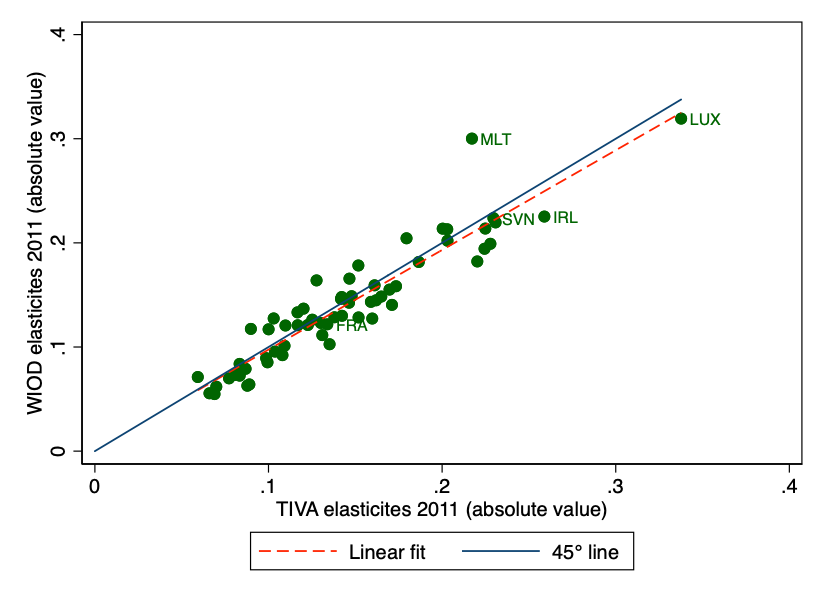
\includegraphics[width=3in, height=2in]{Comparaison_WIOD_TIVA_2011.png}
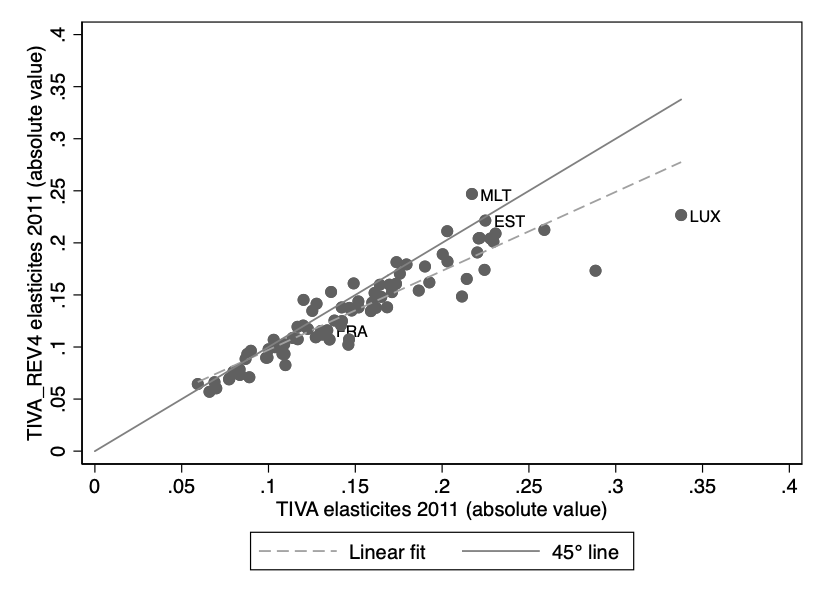
\includegraphics[width=3in, height=2in]{Comparaison_TIVA_REV4_TIVA_2011.png}\\
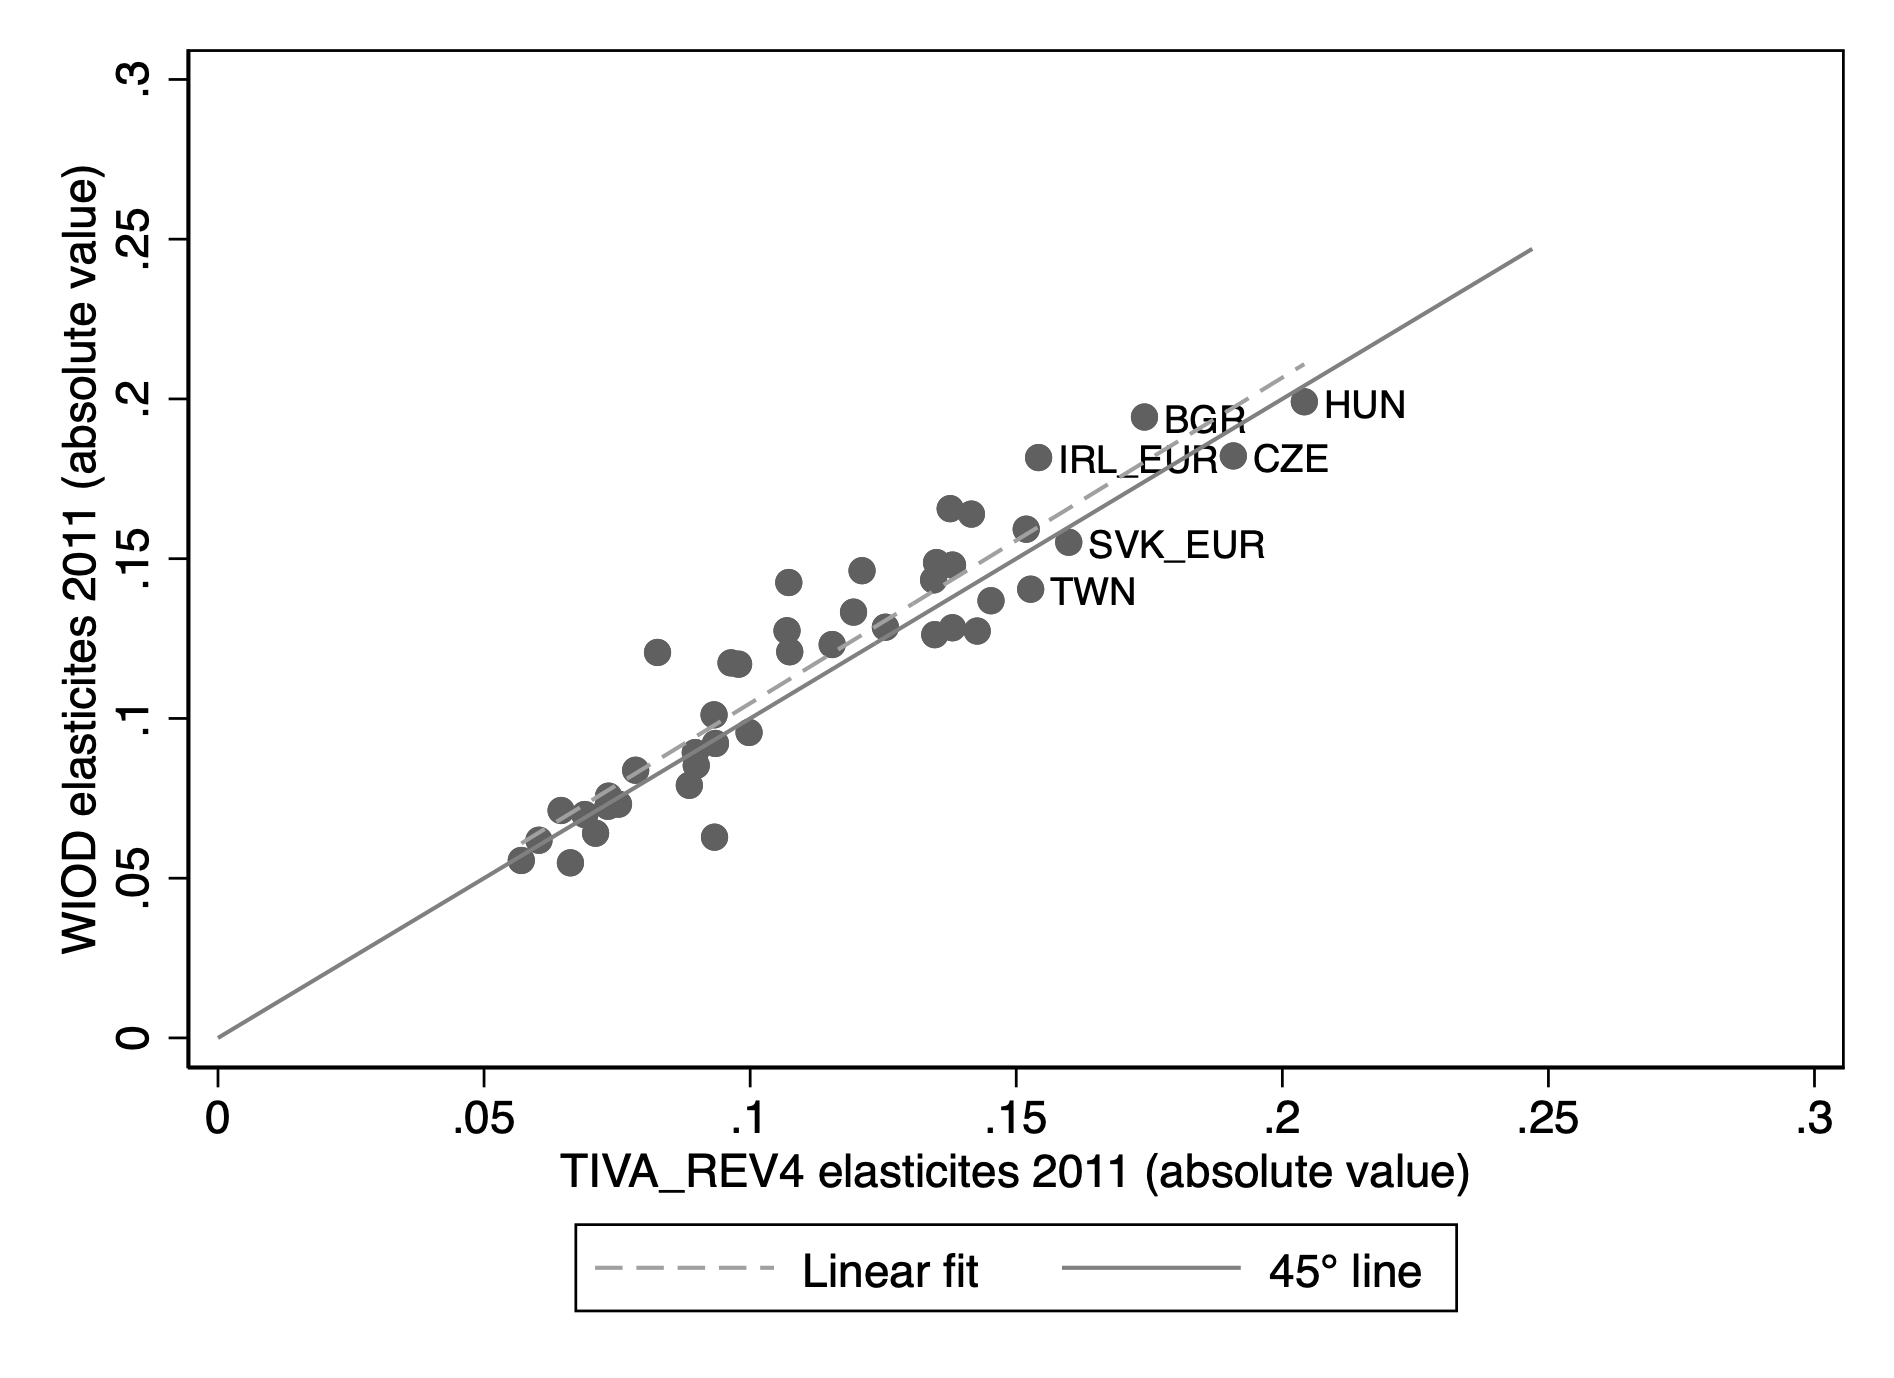
\includegraphics[width=3in, height=2in]{Comparaison_WIOD_TIVA_REV4_2011.png}
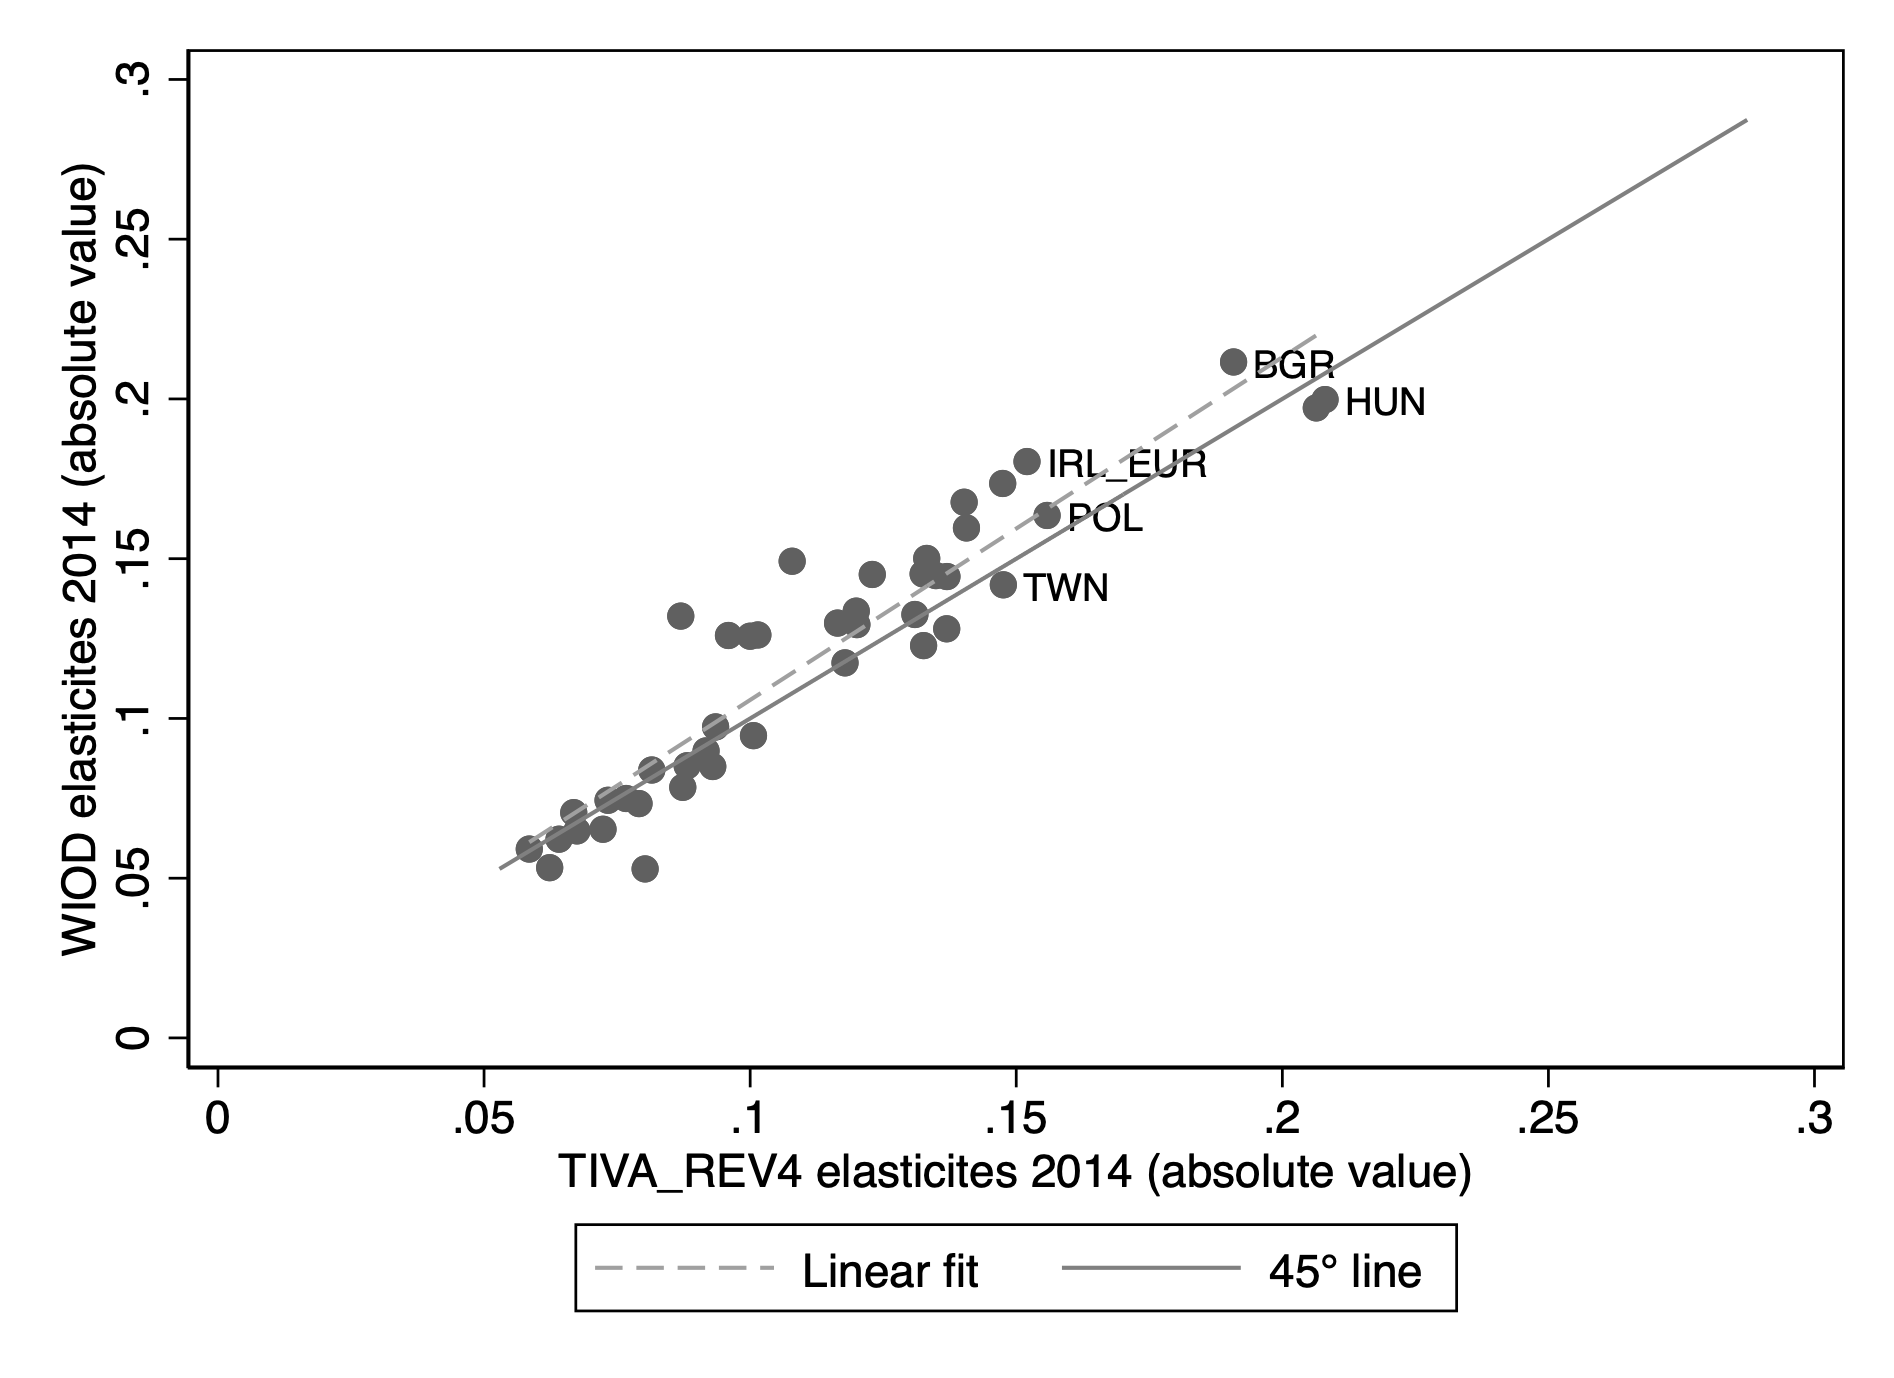
\includegraphics[width=3in, height=2in]{Comparaison_WIOD_TIVA_REV4_2014.png}\\
\floatfoot{Sources: WIOD, TIVA rev3 and TIVA rev4, authors’ calculations}.
\end{tabular}
\label{fig:comp_WIOD_TIVA}
\end{figure}


Using a sample of 43 countries, we plot the elasticity of the HCE deflator to the exchange rate over time. The anual evolution is the same regardless of the database (WIOD or TIVA).
Using data from TIVA rev. 3 yields a higher elasticity  (see Figure \ref{fig:PIWIM_LONGITUDINAL}): it can be explained by different treatment of contract manufacturing in the 2008 system of national accounts compared to the 1993 one which reduces imported inputs.
The small difference between WIOD and TiVA rev. 4 comes maybe from their different ways of reconciling national accouts and international trade statistics.
Output-weighed results show a lower elasticity, reflecting the fact that large countries are relatively closed compared to small economies.
Based on the third revision of TiVA database, we find that the output-weighed elasticity has increased by 25\% between 1995 and 2008, reaching 0.1 in 2008. 
The elasticity has slightly declined afterwards.\\

\begin{figure}[H]
	\centering
	\caption{\footnotesize{\textbf{Comparison of the average HCE deflator elasticity to an exchange rate shock in the whole sample for WIOD and TIVA, 1995-2015}}}
	\begin{tabular}{c}
		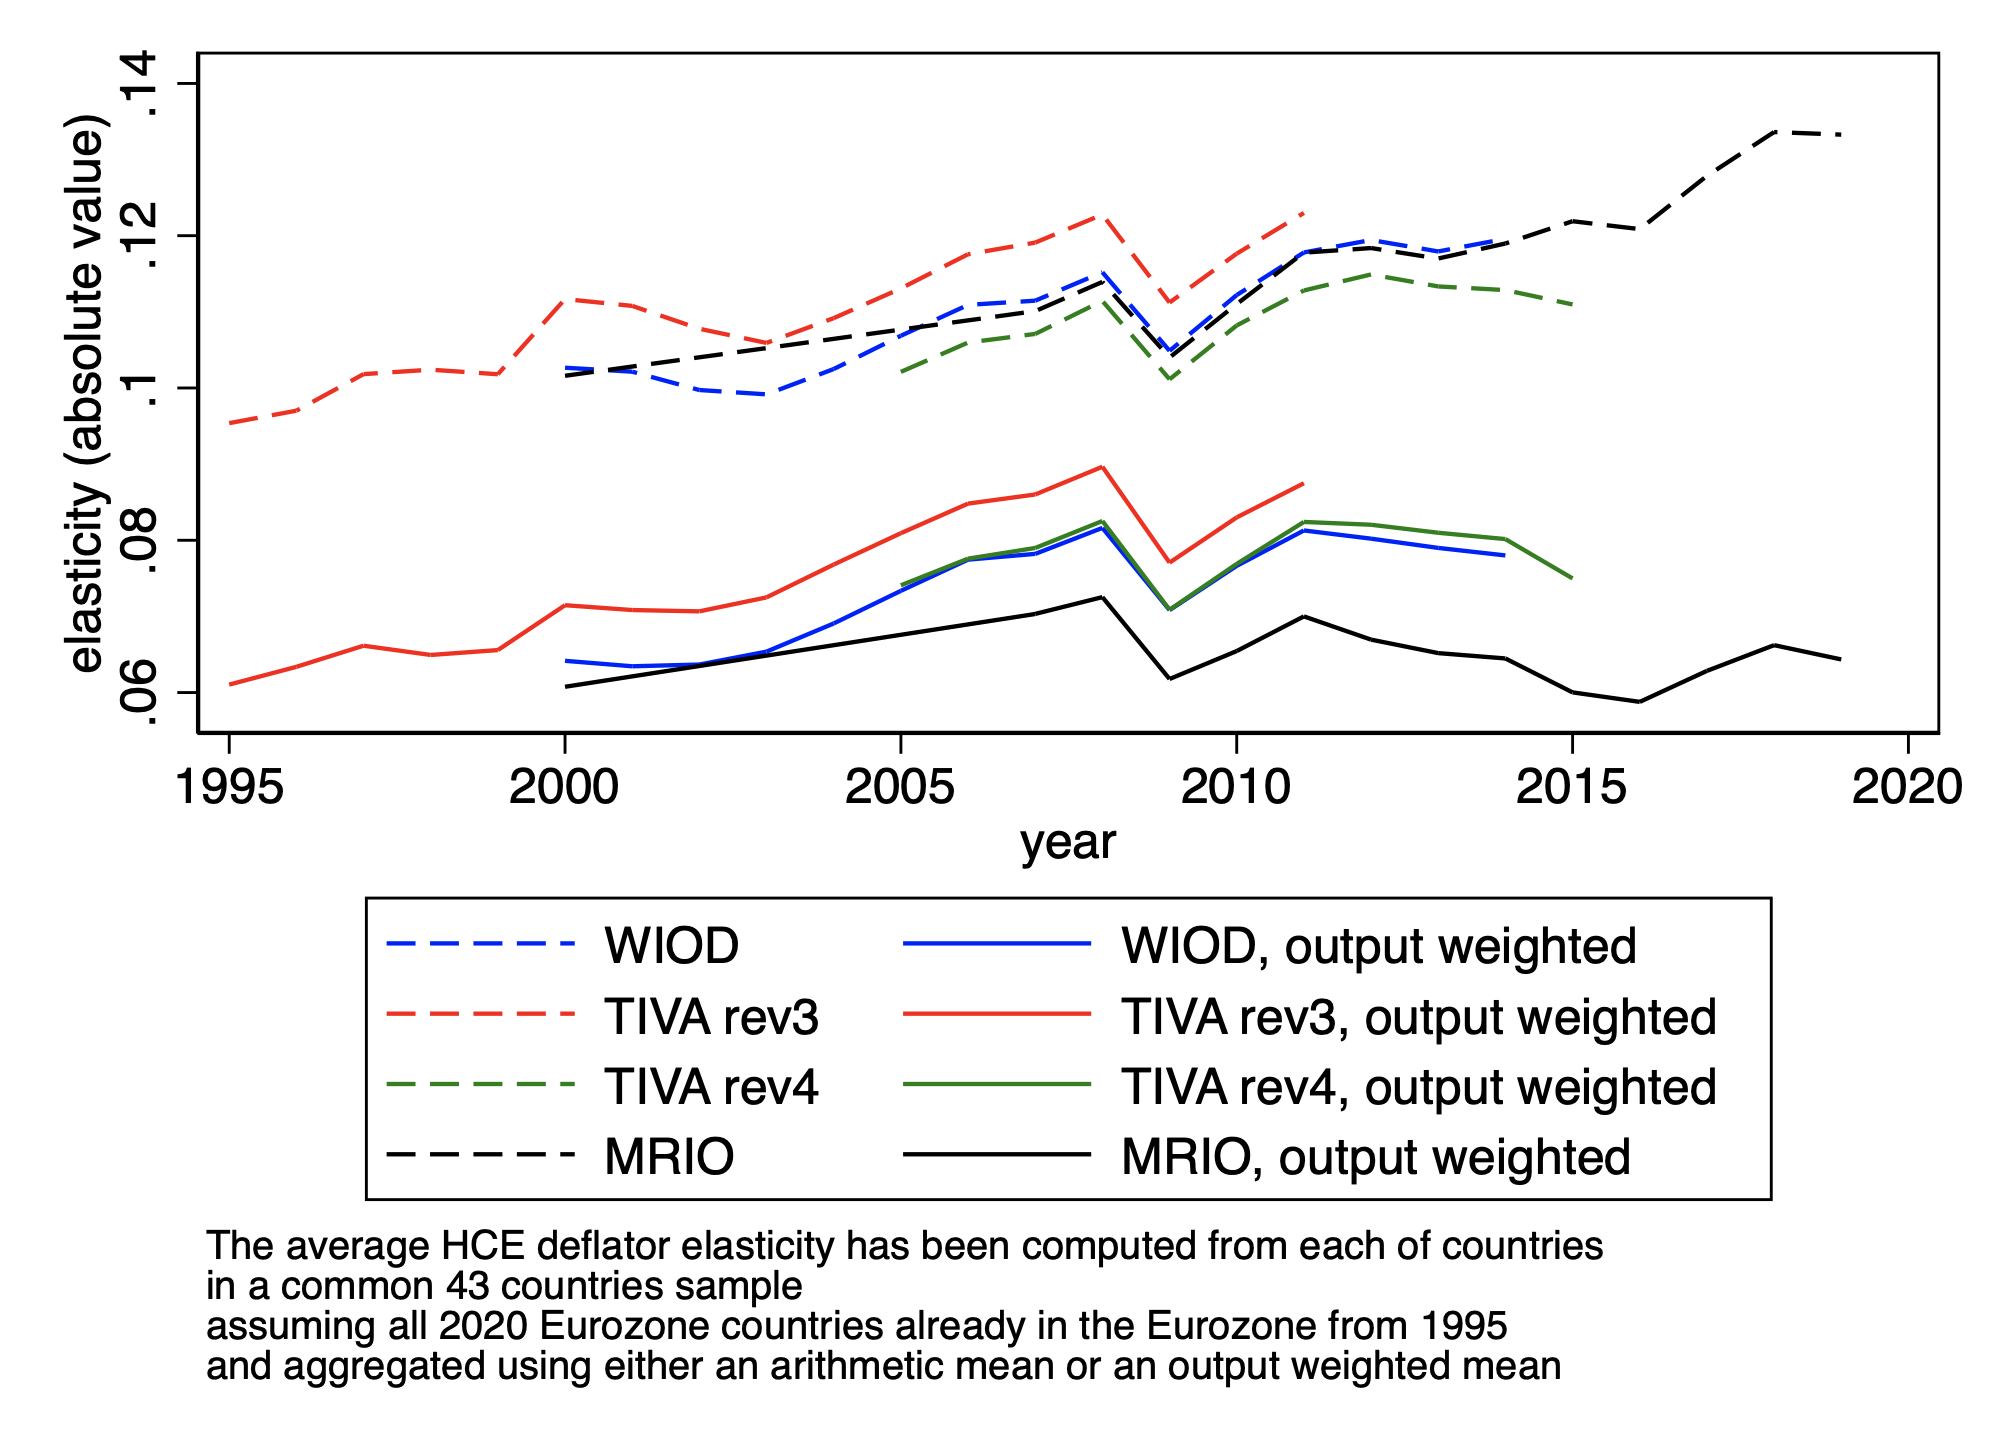
\includegraphics[width=4.5in, height=3in]{PIWIM_LONGITUDINAL.png}\\
		\floatfoot{Sources: WIOD, TIVA rev3, TIVA rev4 and authors’ calculations}
	\end{tabular}
	\label{fig:PIWIM_LONGITUDINAL}
\end{figure}



Using data from WIOD, Figure \ref{fig:WIOD_HC_elasticities} shows that, in absolute terms, the elasticity lies between 0.05 and 0.15, but can be as high as 0.35. 
In the euro area, the elasticity to changes in the value of the euro ranges from 0.065 to 0.18 depending on the member state. This heterogeneity adds to the challenges faced by the European Central Bank in stabilizing prices throughout a monetary union. 
Figure \ref{fig:WIOD_HC_E1HC} shows that the value of the elasticity is closely related to the share of imported goods and services in household consumption.\\

\begin{figure}[H]
	\centering
	\caption{\footnotesize{\textbf{Distribution of the HCE deflator elasticity to an exchange rate shock (WIOD) - 2014.}}}
	\begin{tabular}{c}
		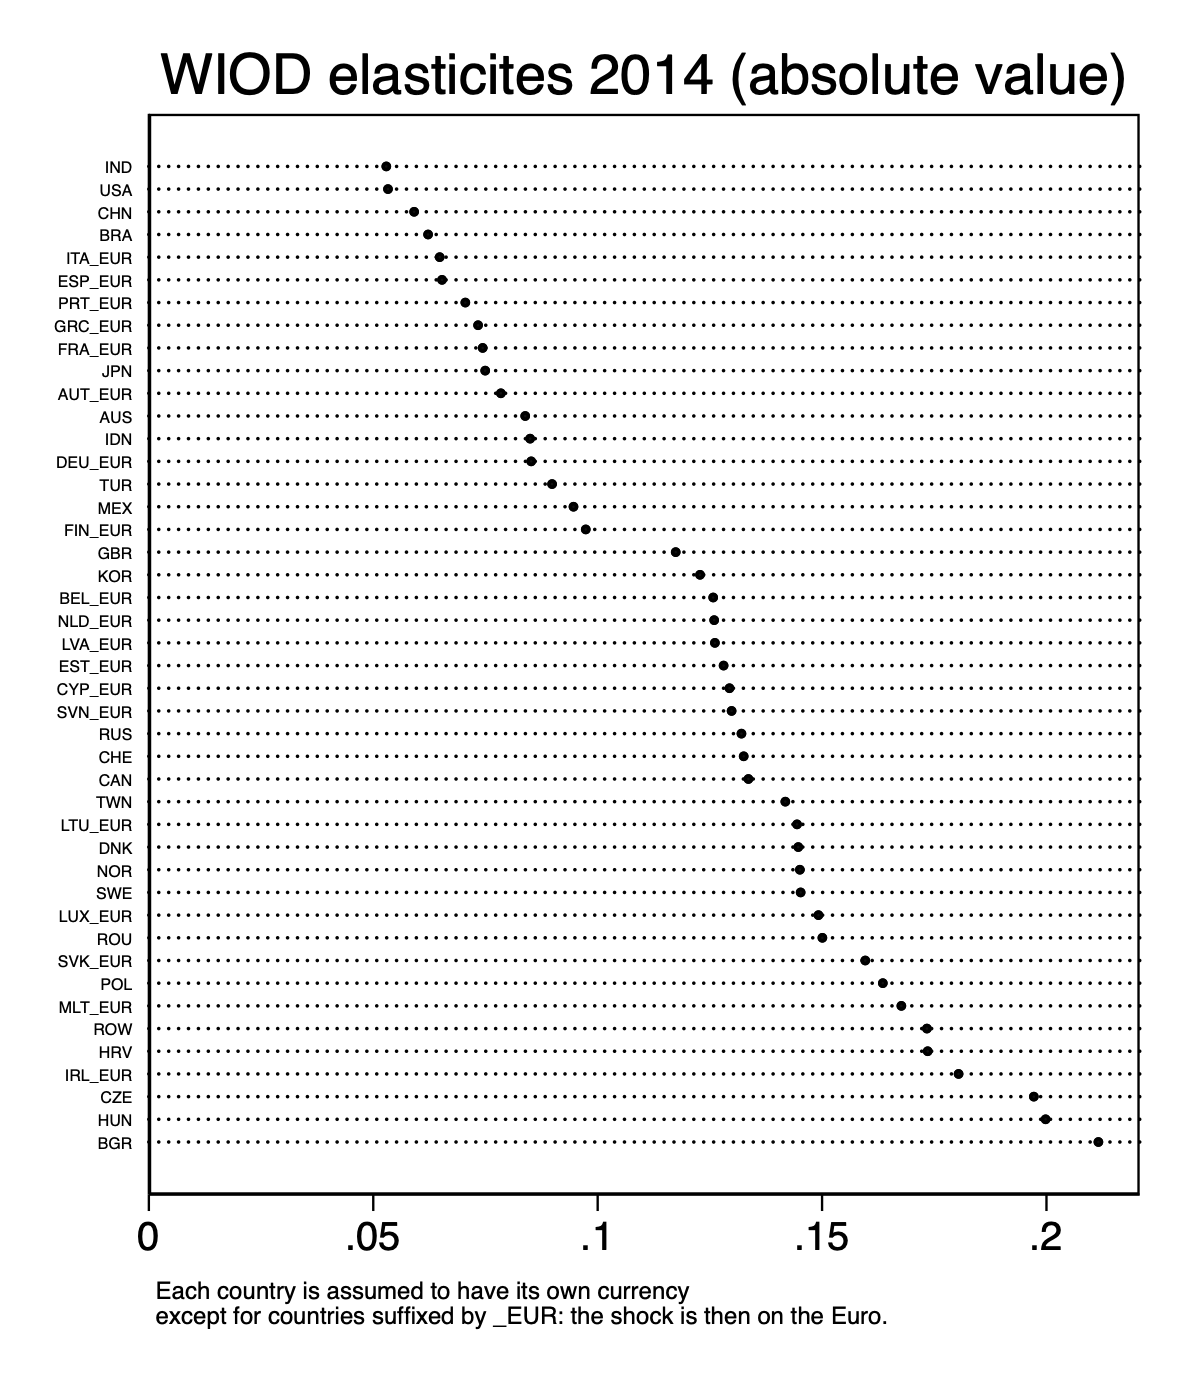
\includegraphics[width=4.5in, height=5.25in]
		{WIOD_HC_elasticities.png}\\
		\floatfoot{Sources: WIOD and authors’ calculations}.
	\end{tabular}
	\label{fig:WIOD_HC_elasticities}
\end{figure}

\begin{figure}[H]
	\centering
	\caption{\footnotesize{\textbf{HCE deflator elasticity to an exchange rate shock and the share of imported consumption in total consumption (WIOD)}}}
	\begin{tabular}{c}
		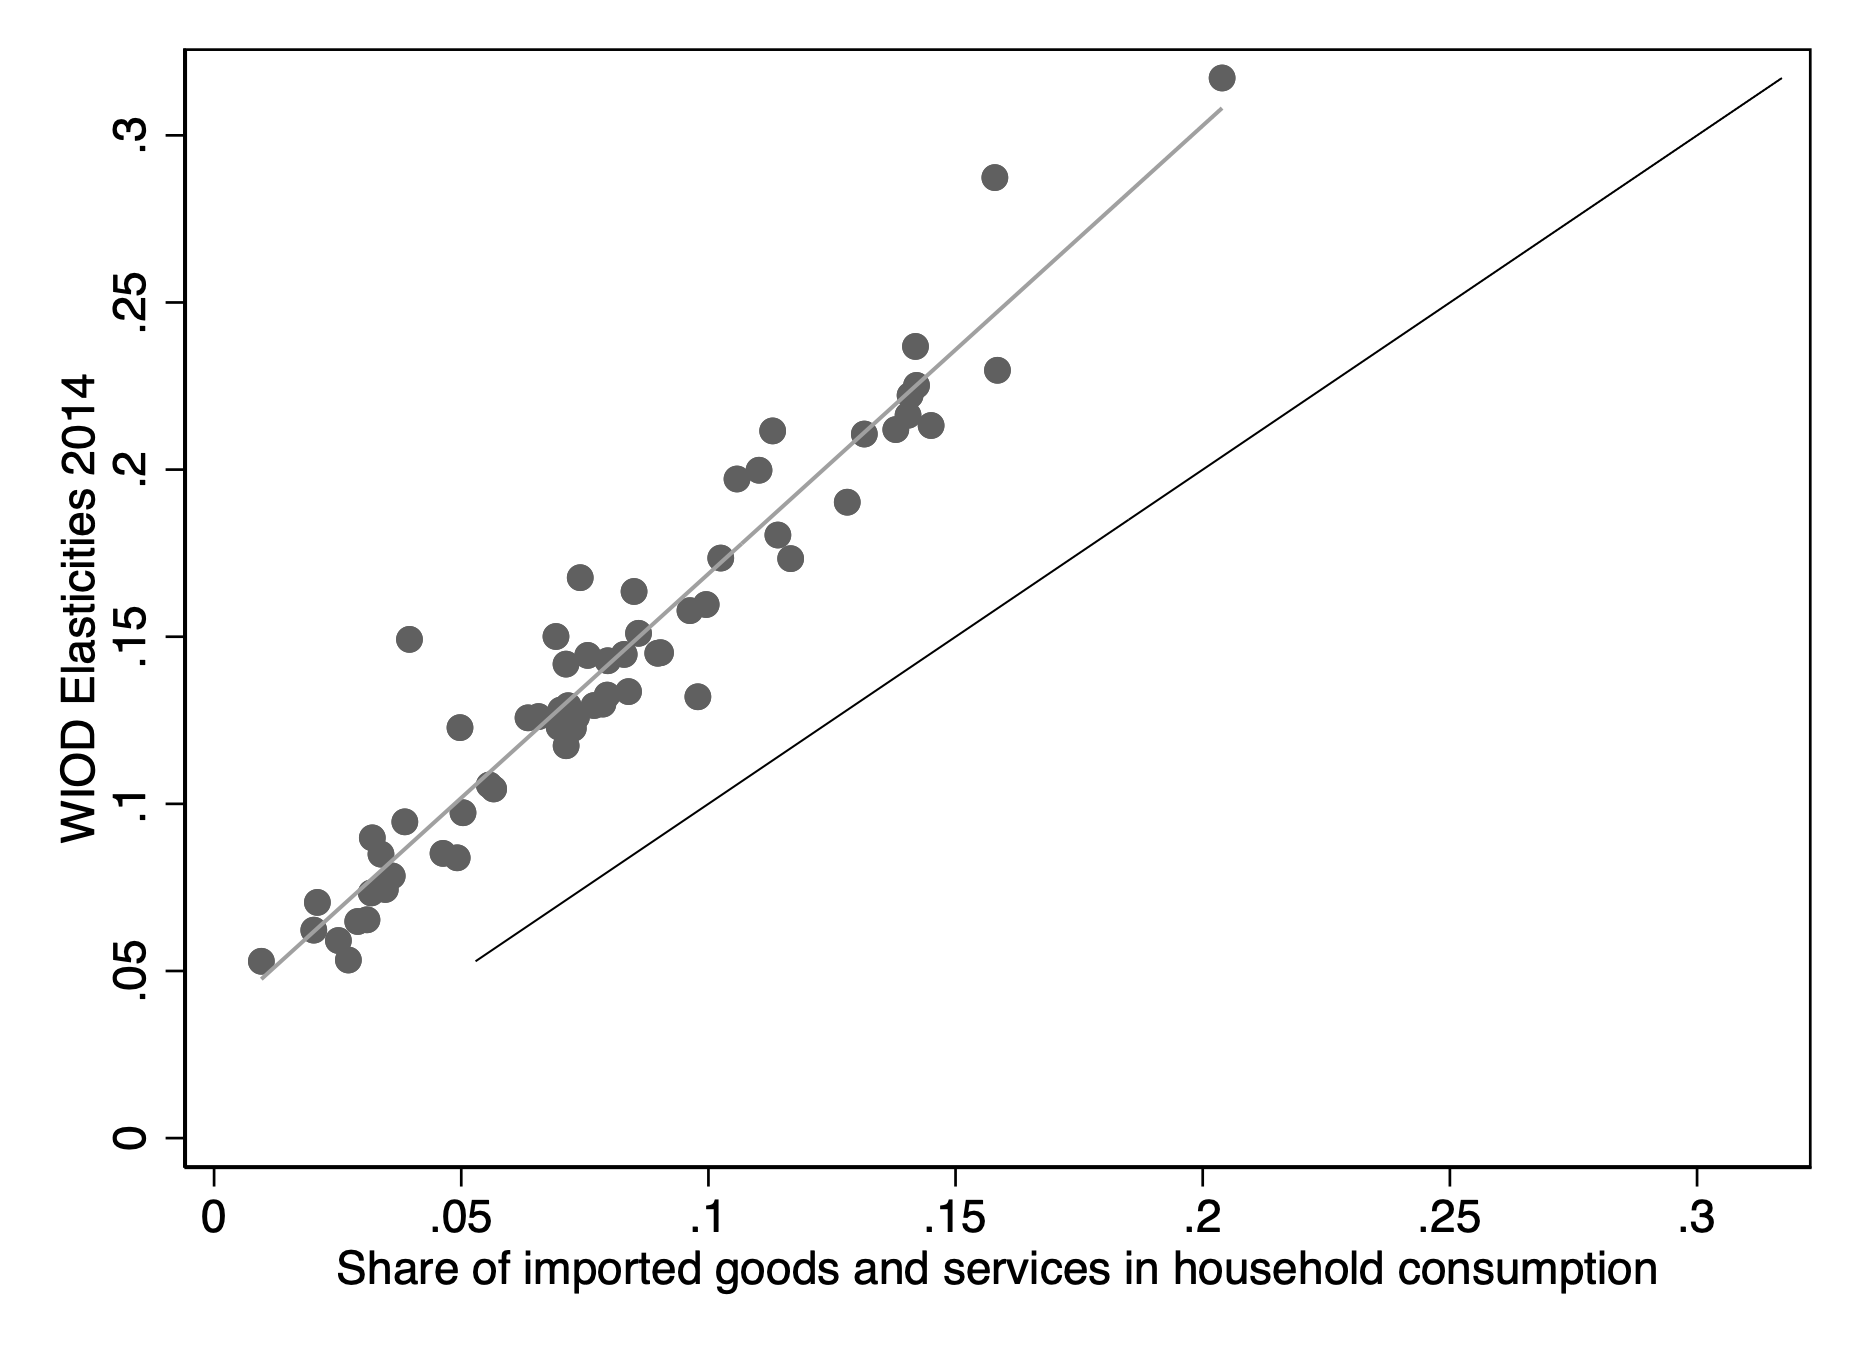
\includegraphics[width=5.0in, height=3.9in]{Comp_s_E1HC_2014_WIOD_HC.png}\\
	\end{tabular}
	\label{fig:WIOD_HC_E1HC}
	\floatfoot{Sources: WIOD and authors’ calculations}
\end{figure}


%
%\begin{figure}[!h]
%	\centering
%	\caption{\footnotesize{\textbf{Consumer price elasticity and share of imported consumption for WIOD 2014}}}
%	\begin{tabular}{c}
%		\includegraphics[width=4.5in, height=3in]
%		{WIOD_HC_E1HC.png}\\
%		\floatfoot{Source: WIOD}.
%	\end{tabular}
%	\label{fig:WIOD_HC_E1HC}
%\end{figure}


%peu intelligible, je suggère de ne pas avoir de sous sections \subsection{Contribution of different goods}
Figure \ref{fig:decomp_origine} contrasts the contribution of domestic versus imported goods to the HCE deflator elasticity to an exchange rate shock.
%Looking at the contribution of different types of goods to $\overline{s_{i}}^{i,HC}$ helps understanding the mechanis at work in PIWIM. One possibility is too look at the predicted effect on domestic goods versus imported goods. 
We define 
\begin{eqnarray}
\overline{s}_i^{i,HC}=\overline{s}_{i,imp}^{i,HC} + \overline{s}_{i,dom}^{i,HC} = S^i.HC^{i,dom}+ S^i.HC^{i,imp}
\label{equ:decomp_impexp}
\end{eqnarray}

Where:
\begin{equation}
\begin{array}{ccccc}
HC^i&=&HC^{i,dom} & + &  HC^{i,imp} \\ 
&=&  \left( \begin{array}{c}
	0 \\
	...\\
	\frac{{hc}_{ij}^i}{hc^i}\\
	...\\
	0
	 \end{array}
	 \right)
&+&
\left( 	\begin{array}{c} \frac{{hc}_{11}^i}{hc^i} \\	...\\0\\...\\\frac{{hc}_{IJ}^i}{hc^i}\end{array}\right) 
\end{array}
\end{equation}

For example,
\begin{equation}
\overline{s}_{i,imp}^{i,HC} = \underset{\begin{subarray}{c}j=1 \dots J   \\ k=1 \dots I \\ k \neq i \end{subarray}}{\mathop \sum}\,{{s}_{kj}^i}.\frac{{hc}_{kj}^i}{hc^i}
\label{equ:share_of_imported}
 \end{equation}


Figure \ref{fig:decomp_origine} shows that changes in the prices of imported final consumer goods contribute more to the total effect than changes in the prices of domestic goods.
Although imported final consumer goods account for a smaller share of total consumption than domestic goods, they are the most impacted by the initial exchange rate shock. 
Imported final consumer goods also explain the differences in price elasticities observed between open and less open economies.\\

\begin{figure}[H]
	\centering
	\caption{\footnotesize{\textbf{Contribution of imported and domestic final goods and services to the HCE deflator elasticity to an exchange rate shock}}}
	\begin{tabular}{c}
		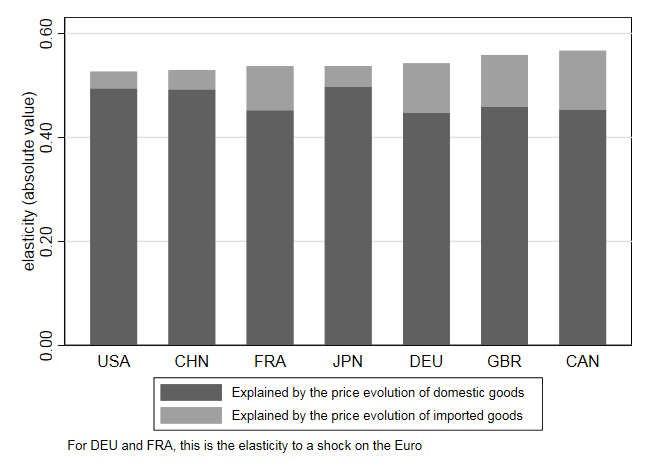
\includegraphics[width=4.5in, height=3in]
		{decomp_origine_WIOD_2014.png}\\
		\floatfoot{Sources: WIOD and authors’ calculations}.
	\end{tabular}
	\label{fig:decomp_origine}
\end{figure}

Figure \ref{fig:decomp_sect} analyses the impact of global inflationary shocks on the main components of the HCE deflator (manufacturing goods, services, food and energy).
Non-energy industrial goods make the bulk of the total impact.
However, services also play a significant role, especially in advanced economies. 
Although services are mainly produced domestically and do not rely much on imported inputs, they make up a substantial share of total consumption.
Similarly, domestic core inflation (all products except food and energy) accounts for a significant share of the total impact (Figure \ref{fig:decomp_sectxorigin}), reflecting the weight of domestic services and non-energy industrial goods in total consumption.
% title Figure 5: contribution of imported and domestic final goods and services to the CPI elasticity to an exchange rate shock
% title Figure 6: contribution of different products to the CPI elasticity to an exchange rate shock
%A major part of the shock comes from lower prices for service consumption (Figure \ref{fig:decomp_sect}). This is paradoxical since, on the one hand, services are not imported a lot and, on the other hand, domestic services do not use many imported inputs. Similarly, domestic core inflation accounts for most of the shock effect for the same reason (Figure \ref{fig:decomp_sectxorigin}). These two phenomena can be explained by the significant weight in the consumption of services on the one hand and domestic services and non-energy industrial goods on the other hand.



\begin{figure}[H]
	\centering
	\caption{\footnotesize{\textbf{Contribution of different products to the HCE deflator elasticity to an exchange rate shock}}}
	\begin{tabular}{c}
		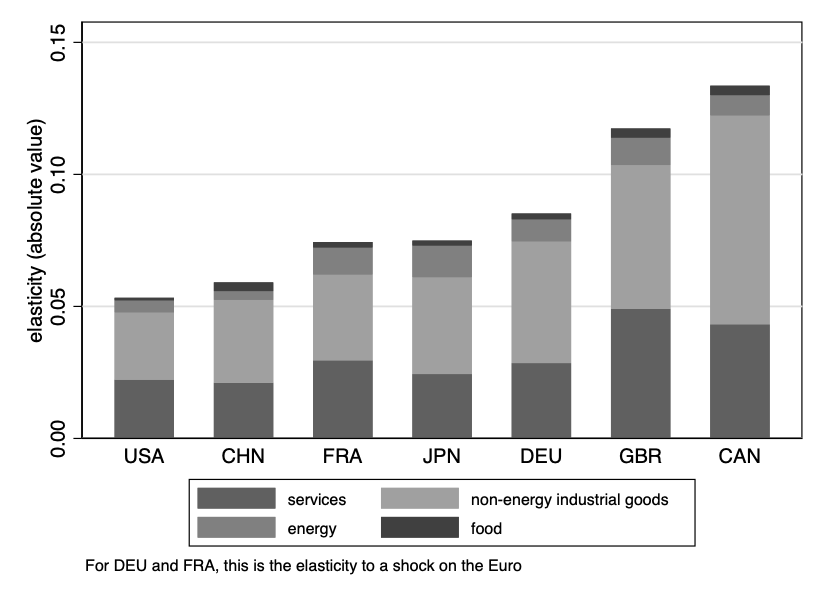
\includegraphics[width=4.5in, height=3in]
		{decomp_sect.png}\\.
	\end{tabular}
	\floatfoot{Sources: WIOD and authors’ calculations}
	\label{fig:decomp_sect}
\end{figure}



\begin{figure}[H]
	\centering
	\caption{\footnotesize{\textbf{Contribution of domestic and imported components to the HCE deflator elasticity}}}
	\begin{tabular}{c}
		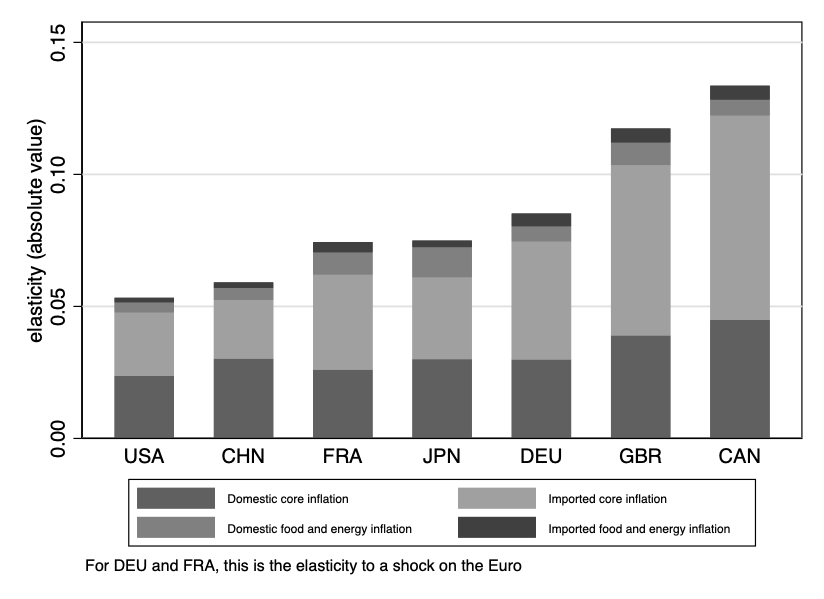
\includegraphics[width=4.5in, height=3in]
		{decomp_sectxorigin.png}\\
		\floatfoot{Sources: WIOD and authors’s calculations}.
	\end{tabular}
	\label{fig:decomp_sectxorigin}
\end{figure}




%
%We can then define the contribution of imported consumption goods to an exchange rate shock as $\nicefrac{\overline{s}_{i,imp}^{i,HC}}{\overline{s}_{i}^{i,HC}} = \nicefrac{S^i.HC^{i,imp}}{S^i.HC^{i}}$. We can also define the sensitivity of imported consumption prices as $ \frac{\nicefrac{S^i.HC^{i,imp}}{S^i.HC^{i}}}{\vec{1}.HC^i,imp}$ where $\vec 1$ is a horizontal vector of ones.
%For example, if an appreciation exchange rate reduce household consumption prices by 20\%, that household consumption is 50\% imported and that imported consumption goods prices evolution cause in a reduction of household consumption prices of 15\%, then the contribution of imported consumption goods will be 0.75 (=.15/.20)and their sensitivity of 1.5 (=0.75/0.5).
%
%GD : PEUT-ÊTRE Y A-T-IL UNE MANIÈRE DE SIMPLIFIER L'EXPRESSION DE LA SENSITIVITÉ, MAIS JE NE VOIS PAS COMMENT FAIRE...
%
%Figure \ref{fig:share_impt} shows, for example, that the contribution of imported consumption is higher than 0.5 in most countries. While imported consumption has a smaller share in total consumption, this is over-compensated by the sensitivity of its prices to exchange rate shocks, as show by the comparison of \ref{fig:intensity_dom} and \ref{fig:intensity_impt}.
%
%Similar decompositions of the matrix $HC^i$ can be done to analyse the contribution of different sectors. decompose the effect between sectors. That allows the identification of the contribution of different sectors to the inflation shocks in different countries.
%Figure \ref{fig:share_sector} shows that non-energy industrial goods and services have the highest contribution. Energy is highly sensitive to exchange rate shocks (see \ref{fig:intensity_dom} and \ref{fig:intensity_impt}), but its share in consumption is too small for its contribution to the final effect to be large.
%
%
%
%\begin{figure}[p]
%\RawFloats
%\centering
%\caption{\footnotesize{\textbf{Contribution of imported final consumption to the impact of a nominal exchange rate shock (see eq. \ref{equ:share_of_imported})}}}
%\begin{tabular}{c}
%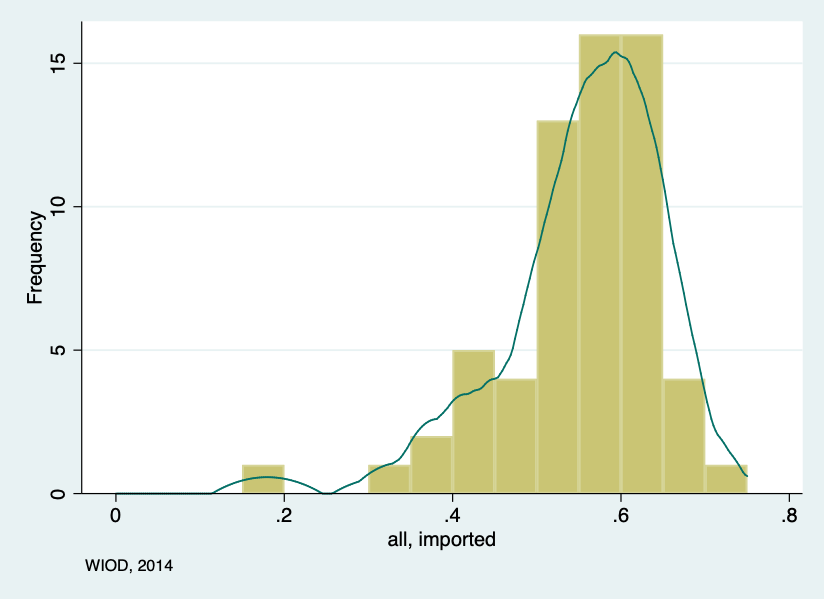
\includegraphics[width=5.0in, height=3.5in]{Share_impt_HC_WIOD_2014.png}\\
%\floatfoot{Interpretation note: the contribution of imported final consumption to the impact of a nominal exchange rate shock is between 55\% and 60\% for 16 countries}
%\end{tabular}
%\label{fig:share_impt}
%
%\caption{\footnotesize{\textbf{Contribution of sector-specific final consumption to the impact of a nominal exchange rate shock}}}
%\begin{tabular}{c}
%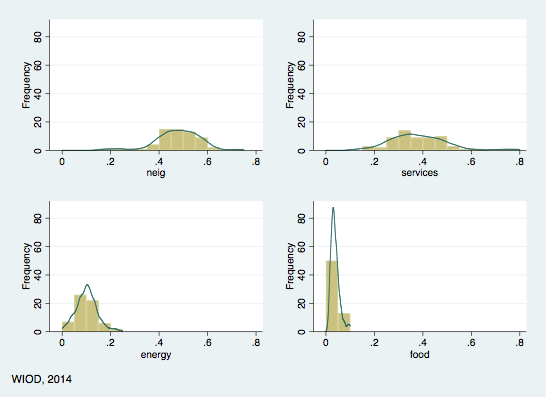
\includegraphics[width=5.0in, height=3.5in]{Share_sector_HC_WIOD_2014.png}\\
%\floatfoot{Interpretation note: the contribution of final energy consumption to the impact of a nominal exchange rate shock is lower than 15\% in most countries}
%\end{tabular}
%\label{fig:share_sector}
%\end{figure}
%
%
%
%
%\begin{figure}[p]
%\RawFloats
%\centering
%\caption{\footnotesize{\textbf{Sensitivity of different domestic sectors to an exchange rate shock}}}
%\begin{tabular}{c}
%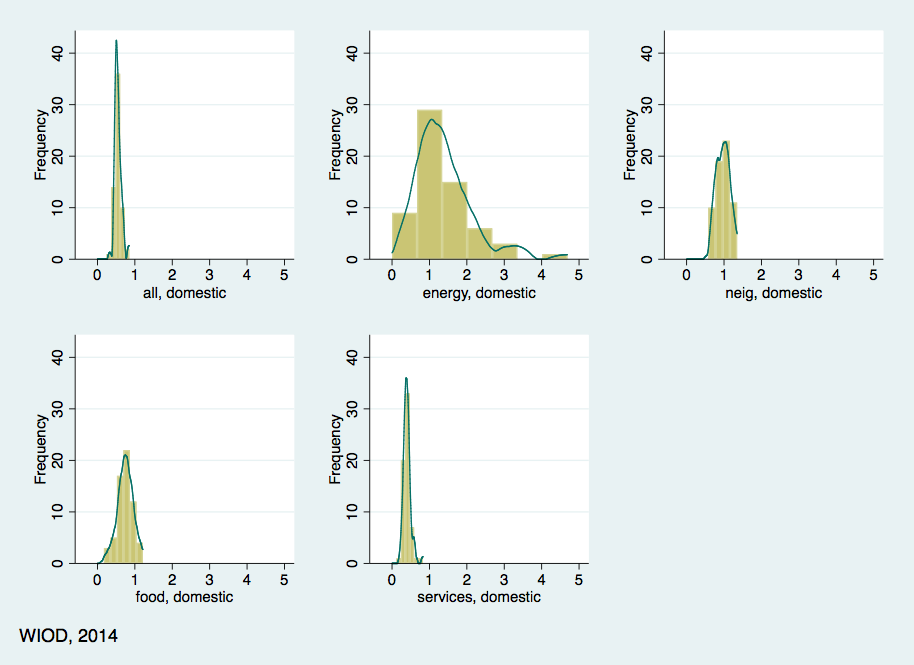
\includegraphics[width=5.0in, height=3.5in]{Int_HC_WIOD_2014_dom.png}\\
%\floatfoot{Intensity is measured as the explained share of inflation change divided by the share in final consumption}
%\end{tabular}
%\label{fig:intensity_dom}
%
%\caption{\footnotesize{\textbf{Sensitivity of imported sectors to an exchange rate shock}}}
%\begin{tabular}{c}
%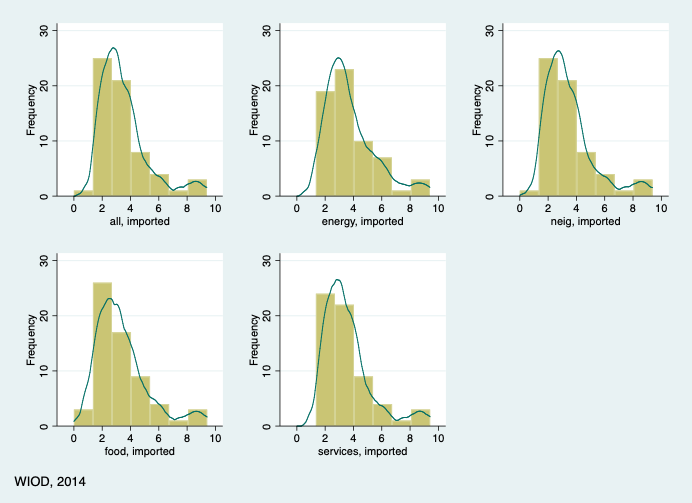
\includegraphics[width=5.0in, height=3.5in]{Int_HC_WIOD_2014_impt.png}\\
%\floatfoot{Intensity is measured as the explained share of inflation change divided by the share in final consumption}
%\end{tabular}
%\label{fig:intensity_impt}
%\end{figure}

\section{Can we extrapolate the HCE deflator elasticity?}
\label{sec:extrapo}
\subsection{Doing without the world input-output matrices}
World input-output matrices are not available for the most recent years: the latest years covered by WIOD and TiVA rev4 are, respectively, 2014 and 2015. 
In addition, using WIOTs involves cumbersome computations.
Given these difficulties, we look for a simpler way to compute the elasticity of the HCE deflator to the exchange rate.
We break down $\overline{s_{i}}^{i,HC}$ into different elements classified by ease of use and computation.
Let us start from equation \ref{eq:eqdomcurrency}.
We have:
\begin{equation}
\begin{array}{lccl}
	S^ i&=&C^i	&+ \left(\hat{C}^i_\$.{\cal B}^i+{C^i}{\tilde{{\cal B}^i}}\right)*{{(I-{\cal A})}^{-1}} \\
	S^i &=&\underbrace{C^i}_{\substack{\text{(E1) direct effect through} \\ \text{ imported consumption goods}}}&+ \underbrace{{C^i}{\tilde{{\cal B}^i}}}_{\substack{\text{(E2) effect on} \\ \text{ \emph{domestic} consumption goods} \\ \text{ through \emph{imported} inputs}}}  + \underbrace{\hat{C}^i_\$.{\cal B}^i}_{\substack{\text{(E3)  effect on} \\ \text{\emph{imported} consumption goods} \\ \text{through \emph{domestic} inputs}}} \\ &&+\underbrace {\left( \hat{C}^i_\$.{\cal B}^i + {C^i}{\tilde{{\cal B}^i}}\right)*{{(I-{\cal A})}^{-1}}*{\cal A}}_{\text{(E4) residual}} \\
\end{array}
\label{eq:decomp}
\end{equation}


$C^i$ and $\hat{C}^i_\$$ have a large number of zeros. So, we can write, defining $HC^{i,dom}$ and $HC^{i,imp}$ as the domestic and imported shares of $HC^i$ and adjusting the dimension of $E1$, $E2$ and $E3$.

\begin{equation}
\begin{array}{lccl}
\overline{s}_{i}^{i,HC}&=S^i.HC^i=E1.HC^i+E2.HC^i+E3.HC^i+E4.HC^i \\
&=E1.HC^{i,imp}+E2.HC^{i,dom}+E3.HC^{i,imp}+E4.HC^i
 \end{array} 
 \label{eq:eqtoto}
 \end{equation}
 
When the domestic currency appreciates, $E1.HC^{i,imp}$ (for short $E1.HC$), $E2.HC^{i,dom}$ (for short $E2.HC$) reduce the consumer prices of the country $i$ whereas $E3.HC^{i,imp}$ (for short $E3.HC$) increases them. 
%je suggère de supprimer le fait qu'il n'y a pas besoin d'inverser de matrice car cette opération est relativement facile avec les logiciels disponibles aujourd'hui

 
This decomposition differs from equation \ref{equ:decomp_impexp}. 
Equation \ref{equ:decomp_impexp} focuses on the contribution of domestic versus imported goods to the HCE deflator elasticity to an exchange rate shock.
By contrast, equation \ref{eq:eqtoto} highlights the transmission channels of the shock.


Figure \ref{fig:decompositionofs} plots the shares of $E1.HC$, $E2.HC$, $E3.HC$ and $E4.HC$ (shortening $E4.HC^i$) in $\overline{s}_{i}^{i,HC}$.  
$E1.HC$ dominates. 
While $E3.HC$ is negligible, $E4.HC$ accounts for 10\% to 30\% of $\overline{s}_{i}^{i,HC}$ for most countries except China.
On the whole, as shown by Figure \ref{fig:shareofs}, input-output mechanisms (i.e. everything but $E1.HC$) explain a large share of the elasticity, especially for large countries or countries of the Eurozone subject to a shock on the Euro. This share has increased until 2013-2014, implying an increasing need of data from WIOTs to perform our computations (see Figure \ref{fig:shareofsthroughtime}).

\begin{figure}[H]
\centering
\caption{\footnotesize{\textbf{Decomposition of $\overline{s}_{i}^{i,HC}$ into E1.HC, E2.HC, E3.HC and E4.HC}}}
%La figure vient de Étude rapport D+I et Bouclage Mondial_oil.do
\begin{tabular}{c}
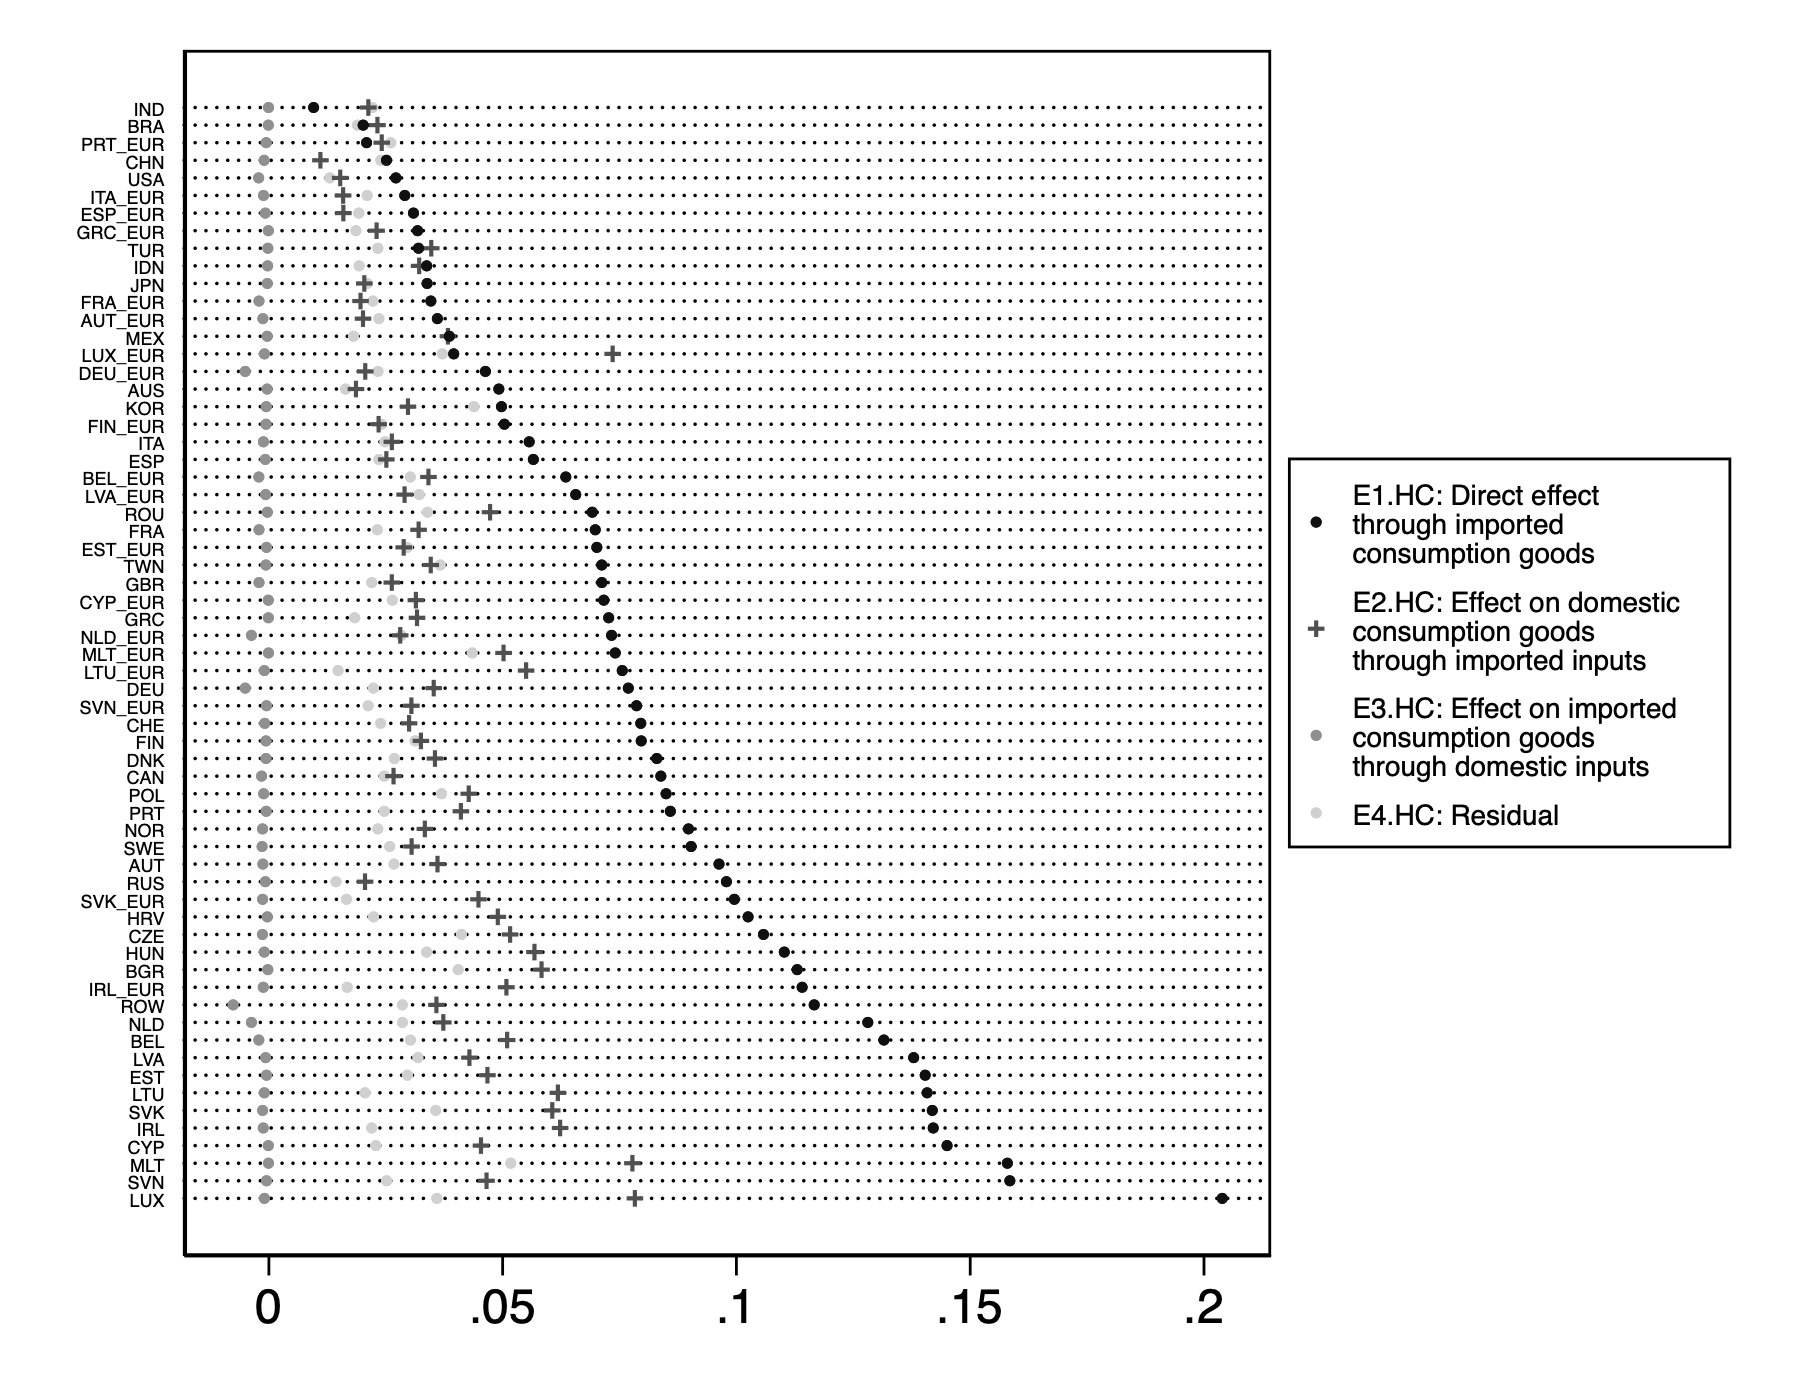
\includegraphics[width=5.0in, height=3.5in]{distribution_components_WIOD_2014.png}\\
\floatfoot{Sources: WIOD and authors’ calculatons}. \\
\end{tabular}
\label{fig:decompositionofs}
\end{figure}


\begin{figure}[H]
	\centering
	\caption{\footnotesize{\textbf{Decomposition of $\overline{s}_{i}^{i,HC}$}}}
	%La figure vient de Étude rapport D+I et Bouclage Mondial_oil.do
	\begin{tabular}{c}
		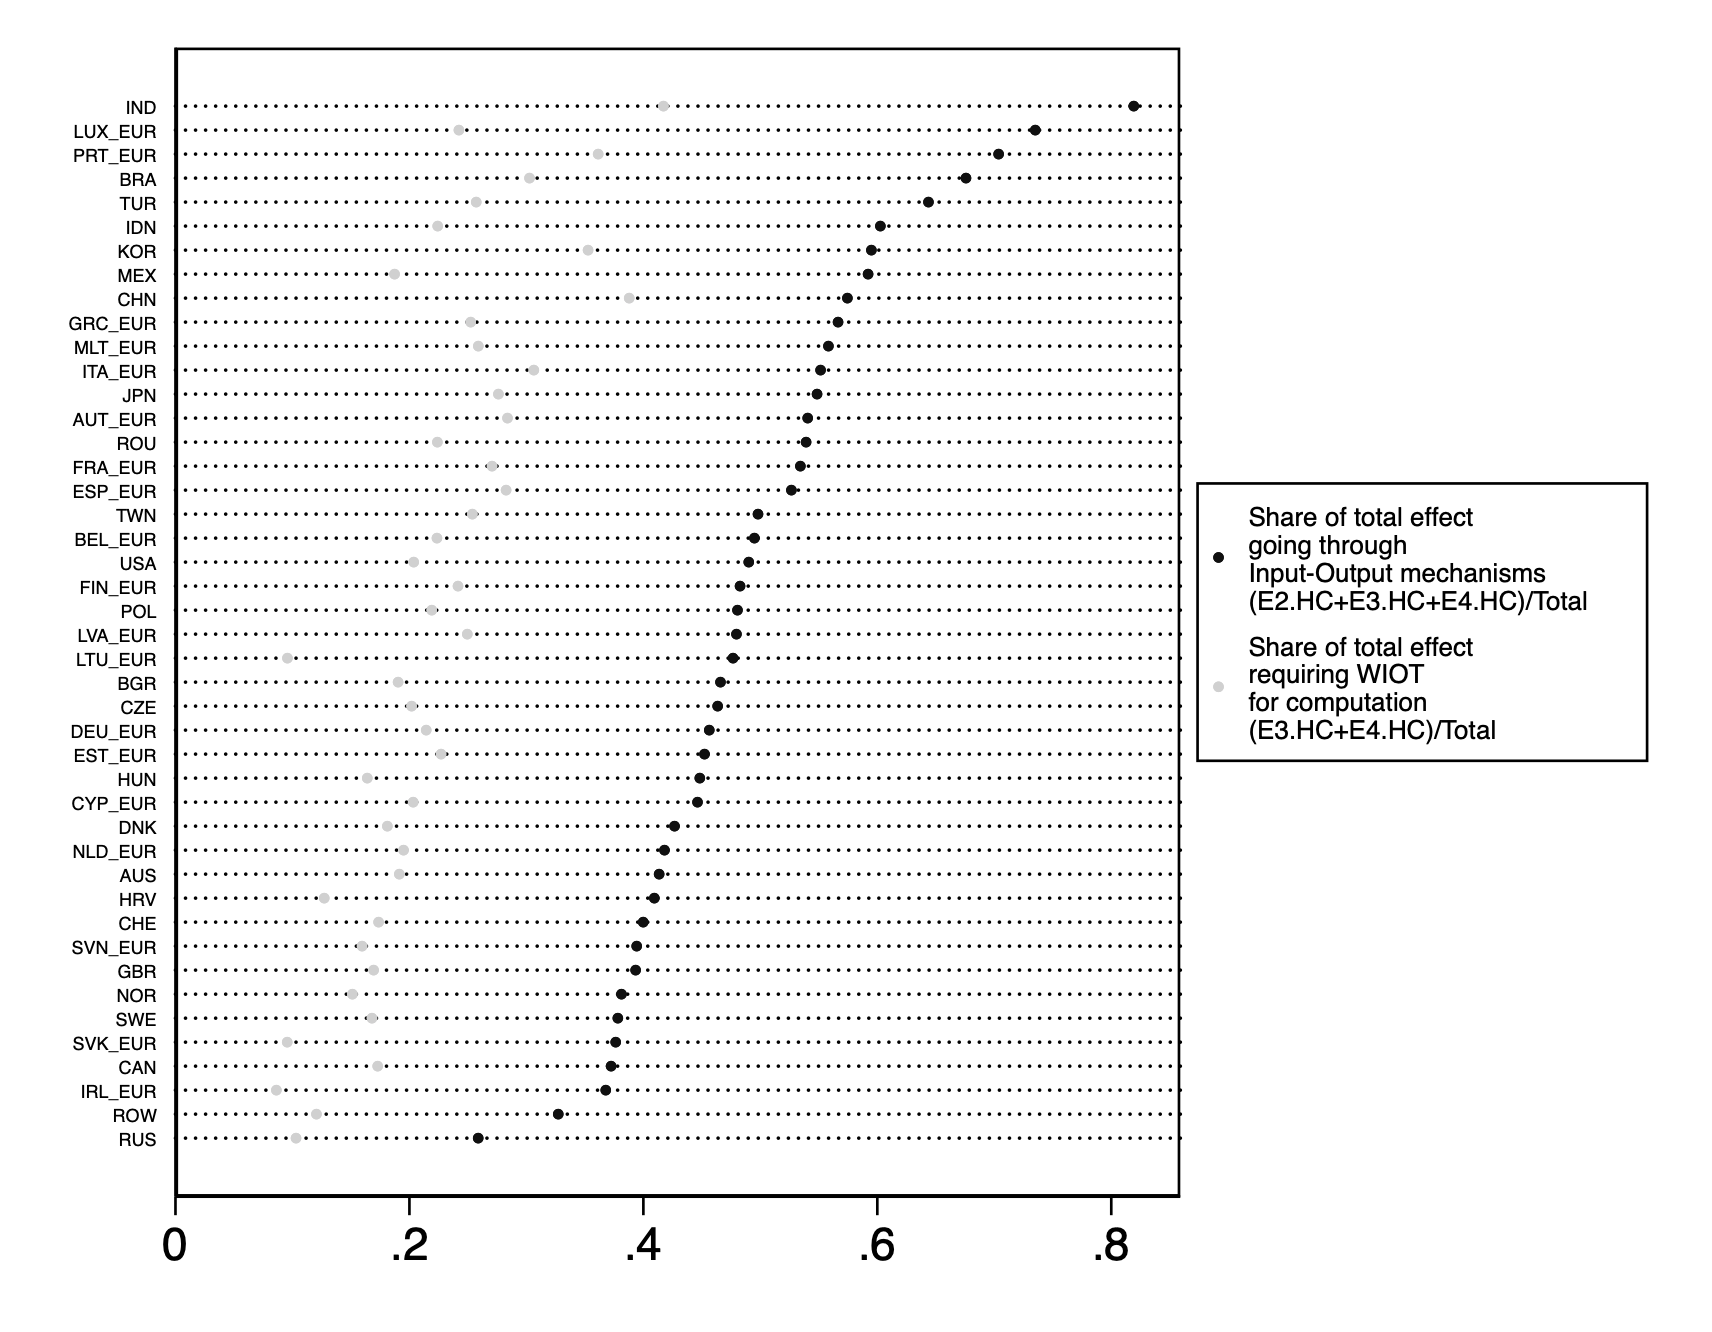
\includegraphics[width=5.0in, height=3.5in]{share_components_WIOD_2014.png}\\
		\floatfoot{Sources: WIOD and authors’ calculations}. \\
	\end{tabular}
	\label{fig:shareofs}
\end{figure}


\begin{figure}[H]
	\centering
	\caption{\footnotesize{\textbf{Decomposition of $\overline{s}_{i}^{i,HC}$ through time}}}
	%La figure vient de Étude rapport D+I et Bouclage Mondial_oil.do
	\begin{tabular}{c}
		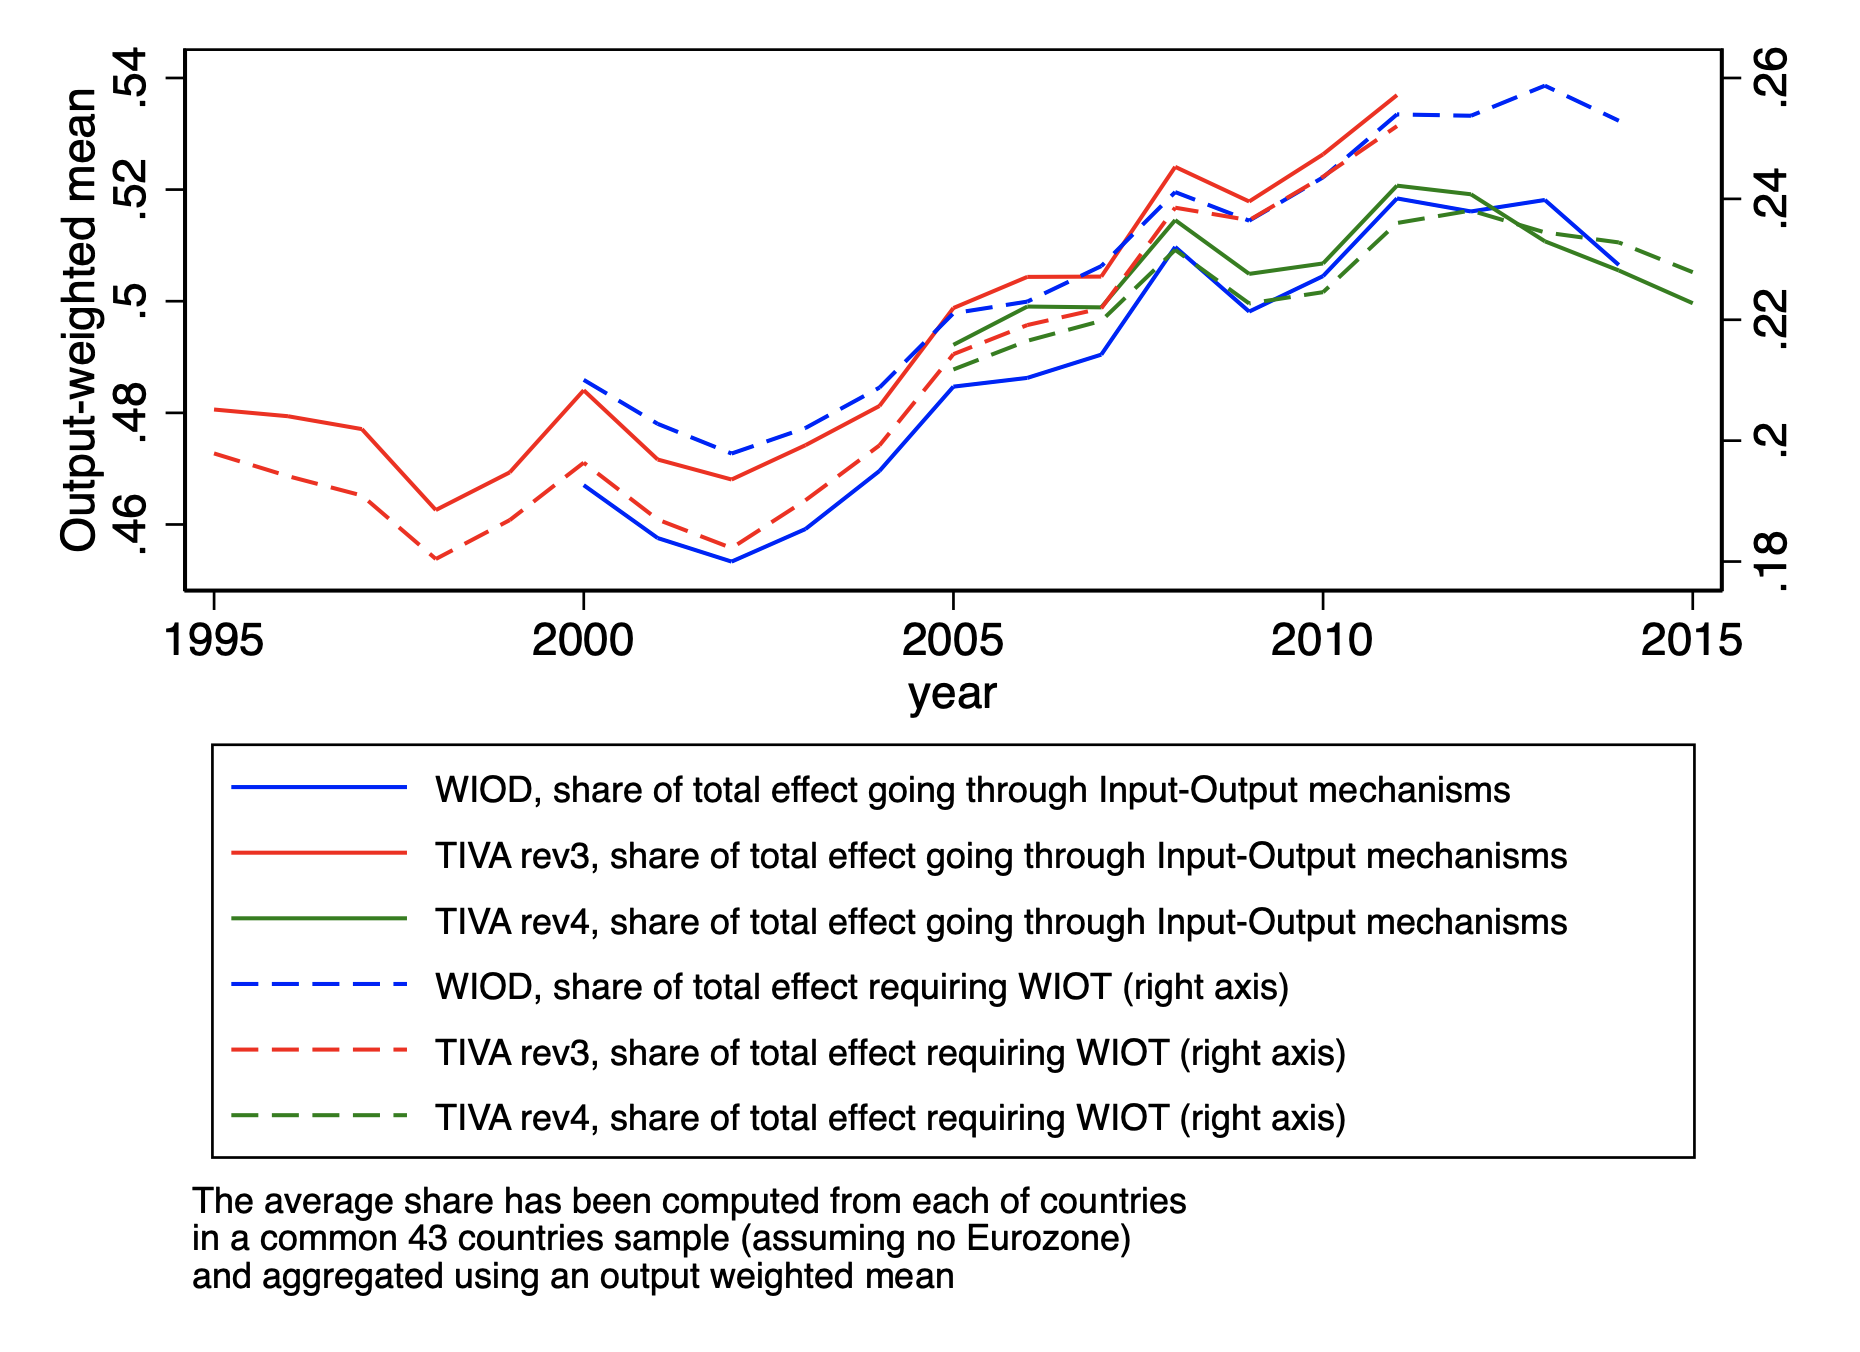
\includegraphics[width=5.0in, height=3.5in]{Share_GDP-weighted.png}\\
		\floatfoot{Sources: WIOD, TIVA rev3, TIVA rev4 and authors’ calculations} \\
	\end{tabular}
	\label{fig:shareofsthroughtime}
\end{figure}

$E1.HC$ and $E2.HC$ can be computed with national input-output matrices whereas world input-output matrices are needed for computing $E3.HC$ and $E4.HC$. 
Although world input-output matrices are not available for the most recent years, $E4.HC$ can be inferred from easier-to-compute elements of $\overline{s}_{i}^{i,HC}$.

%This is suggested by the correlation matrix of  $E1.HC^{i,imp}$, $E2.HC^{i,dom}$, $E3.HC^{i,imp}$ and $E4.HC^i$ (see Table \ref{table:corretable1}). 
%
%\begin{table}[htbp]\centering \caption{Cross-correlation of $\overline{s}_{i}^{i,HC}$'s components (WIOD 2014)\label{table:corretable1}}
\begin{tabular}{l  c  c  c  c }\hline\hline
\multicolumn{1}{c}{Variables} &E1HC&E2HC&E3HC&E4HC\\ \hline
E1HC&1.00\\
E2HC&0.74&1.00\\
E3HC&-0.09&0.11&1.00\\
E4HC&0.36&0.53&0.05&1.00\\
\hline \hline 
 \end{tabular}
\end{table}

% comme on vient de dire que e3 est petit, je sugère de supprimer la phrase ci-dessous
%$E3.HC^{i,imp}$ does not require inverting a matrix, but it is still quite data-intensive to compute. 
We try to infer $\overline{s}_{i}^{i,HC}$ from $E1.HC$ and $E2.HC$.
Figure \ref{fig:ratiodir_WIOD} depicts the relationship between $\overline{s}_{i}^{i,HC}$ and $E1.HC+E2.HC$ according to equation \ref{eq:eq7}. 
The high $R^2$ (0.98) suggests that $E1.HC+E2.HC$ is a good predictor of $\overline{s}_{i}^{i,HC}$. 

 \begin{equation}
\overline{s}_{i}^{i,HC}=\alpha + \beta  \left(E1.HC^{i,imp}+E2.HC^{i,dom}\right) +\varepsilon_i 
\label{eq:eq7}
 \end{equation}
 


\begin{figure}[H]
\centering
\caption{\footnotesize{\textbf{Comparison of $\overline{s}_{i}^{i,HC}$ and $E1.HC^{i,imp}+E2.HC^{i,dom}$}}}
\begin{tabular}{c}
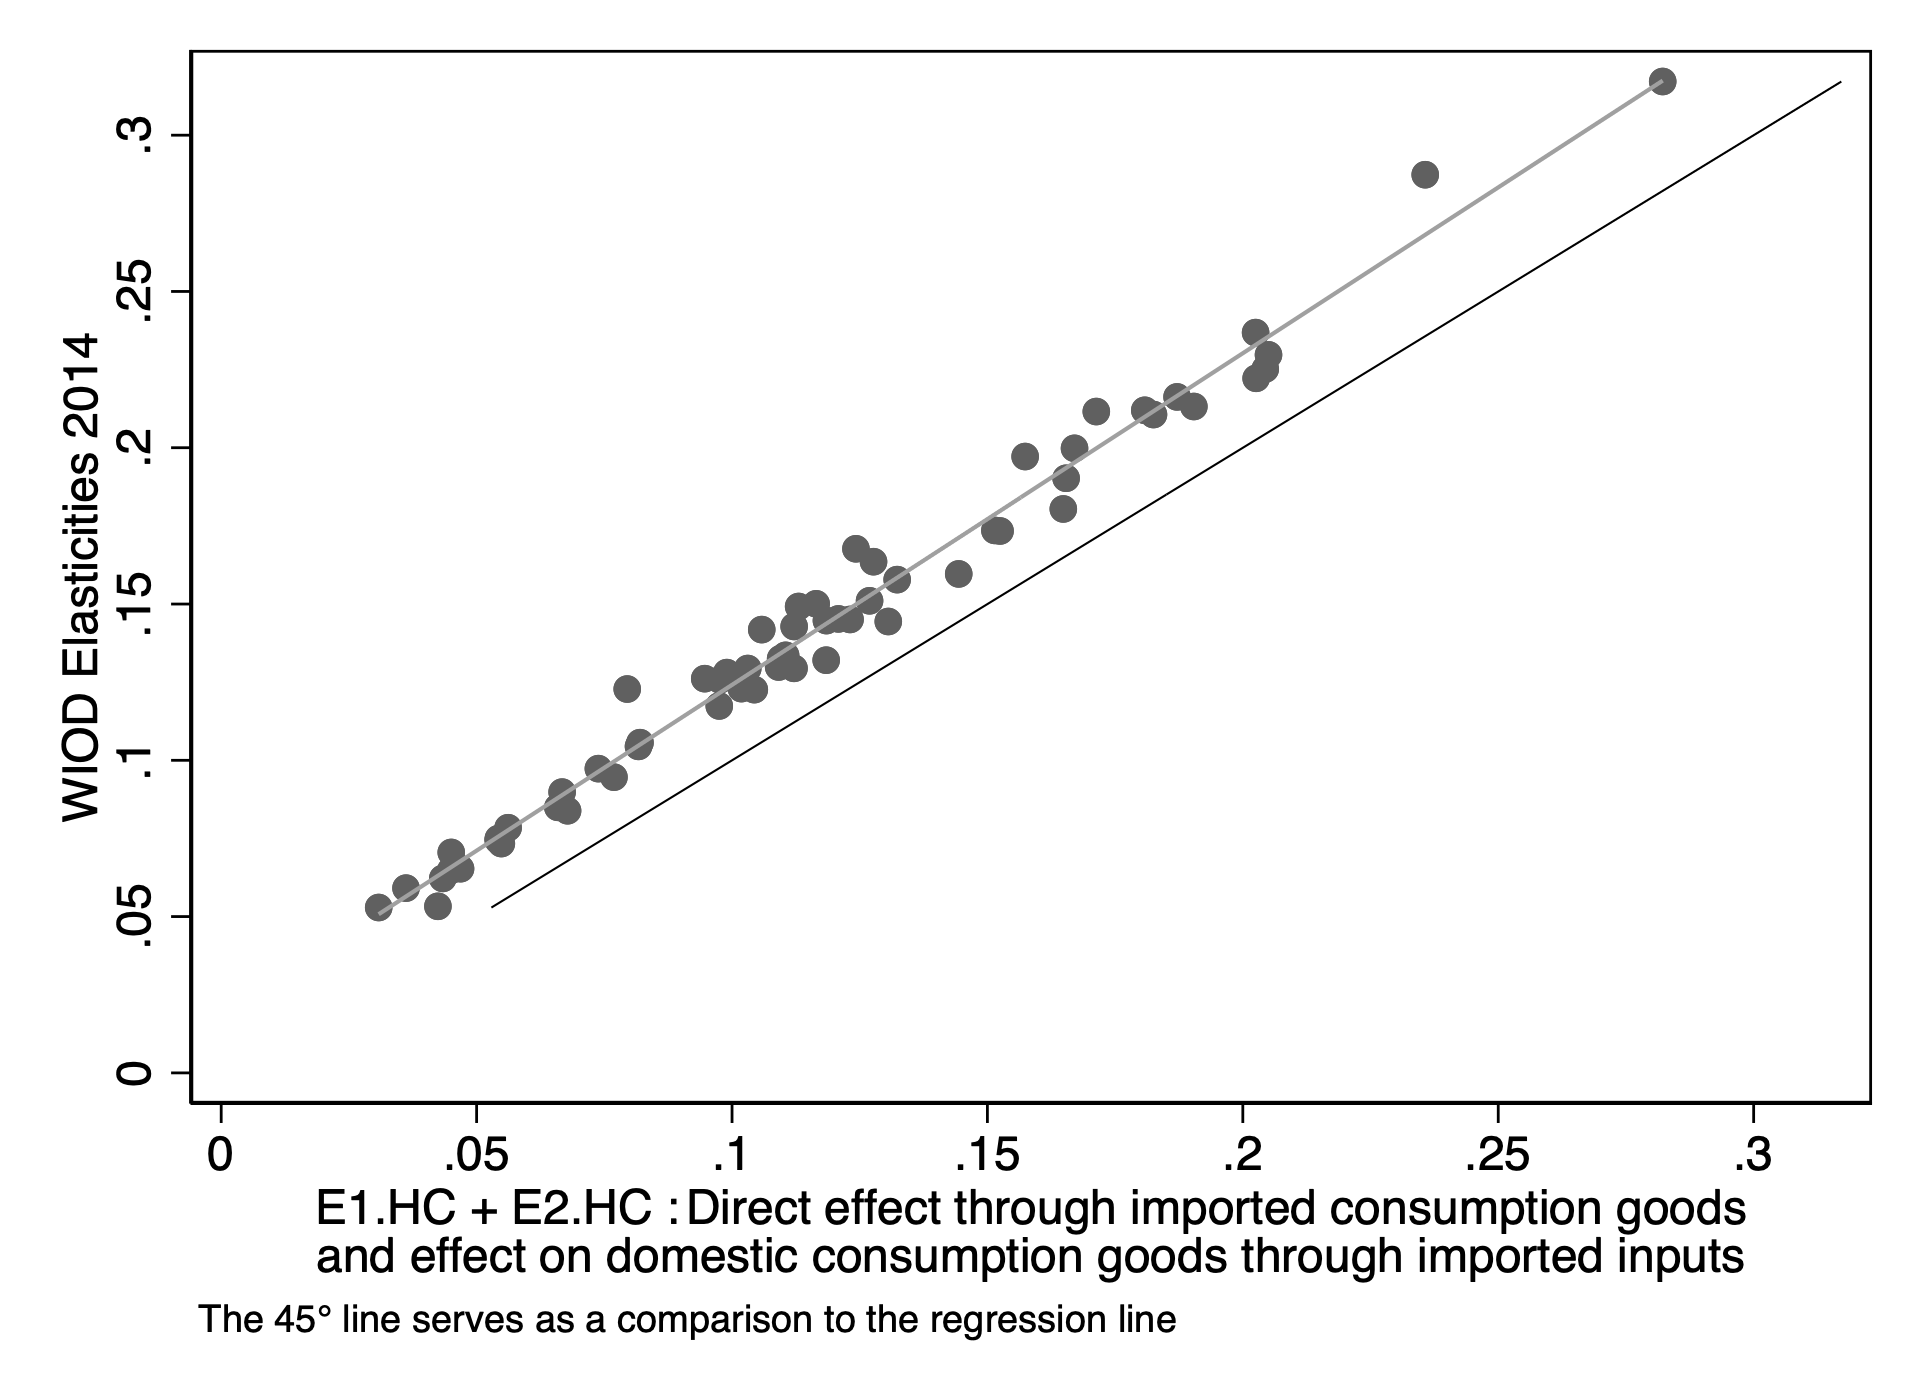
\includegraphics[width=5.0in, height=3.5in]{Comp_s_E1HCE2HC_2014_WIOD_HC.png}\\
\end{tabular}
\floatfoot{Sources: WIOD and authors’ calculations}
\label{fig:ratiodir_WIOD}
\end{figure}

We check whether the relationship is constant over time by estimating yearly cross-sections of equation \ref{eq:eq7}. 
With the exception of 2009, the relationship is broadly stable (see Figures \ref{fig:evolution_b} and \ref{fig:evolution_cst}).

\begin{figure}[H]
\centering
\caption{\footnotesize{\textbf{Evolution of $\beta$ (the coefficent of E1.HC+E2.HC) and $R^2$ over time (WIOD)}}}
\begin{tabular}{c}
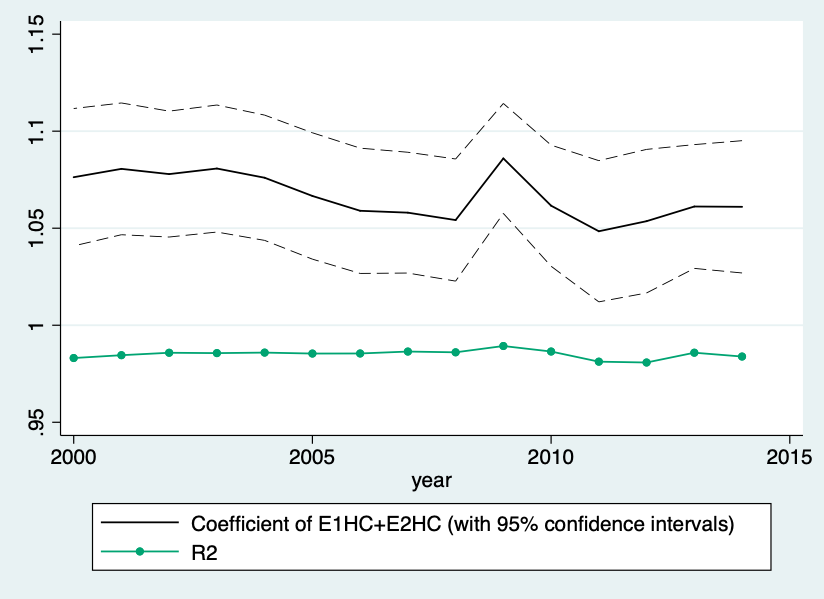
\includegraphics[width=5.0in, height=3.5in]{coef_E_WIOD_HC.png}\\
\end{tabular}
\label{fig:evolution_b}
\floatfoot{Sources: WIOD and authors’ calculations}
\end{figure}

\begin{figure}[H]
\centering
\caption{\footnotesize{\textbf{Evolution of $\alpha$ (the constant) over time (WIOD)}}}
\begin{tabular}{c}
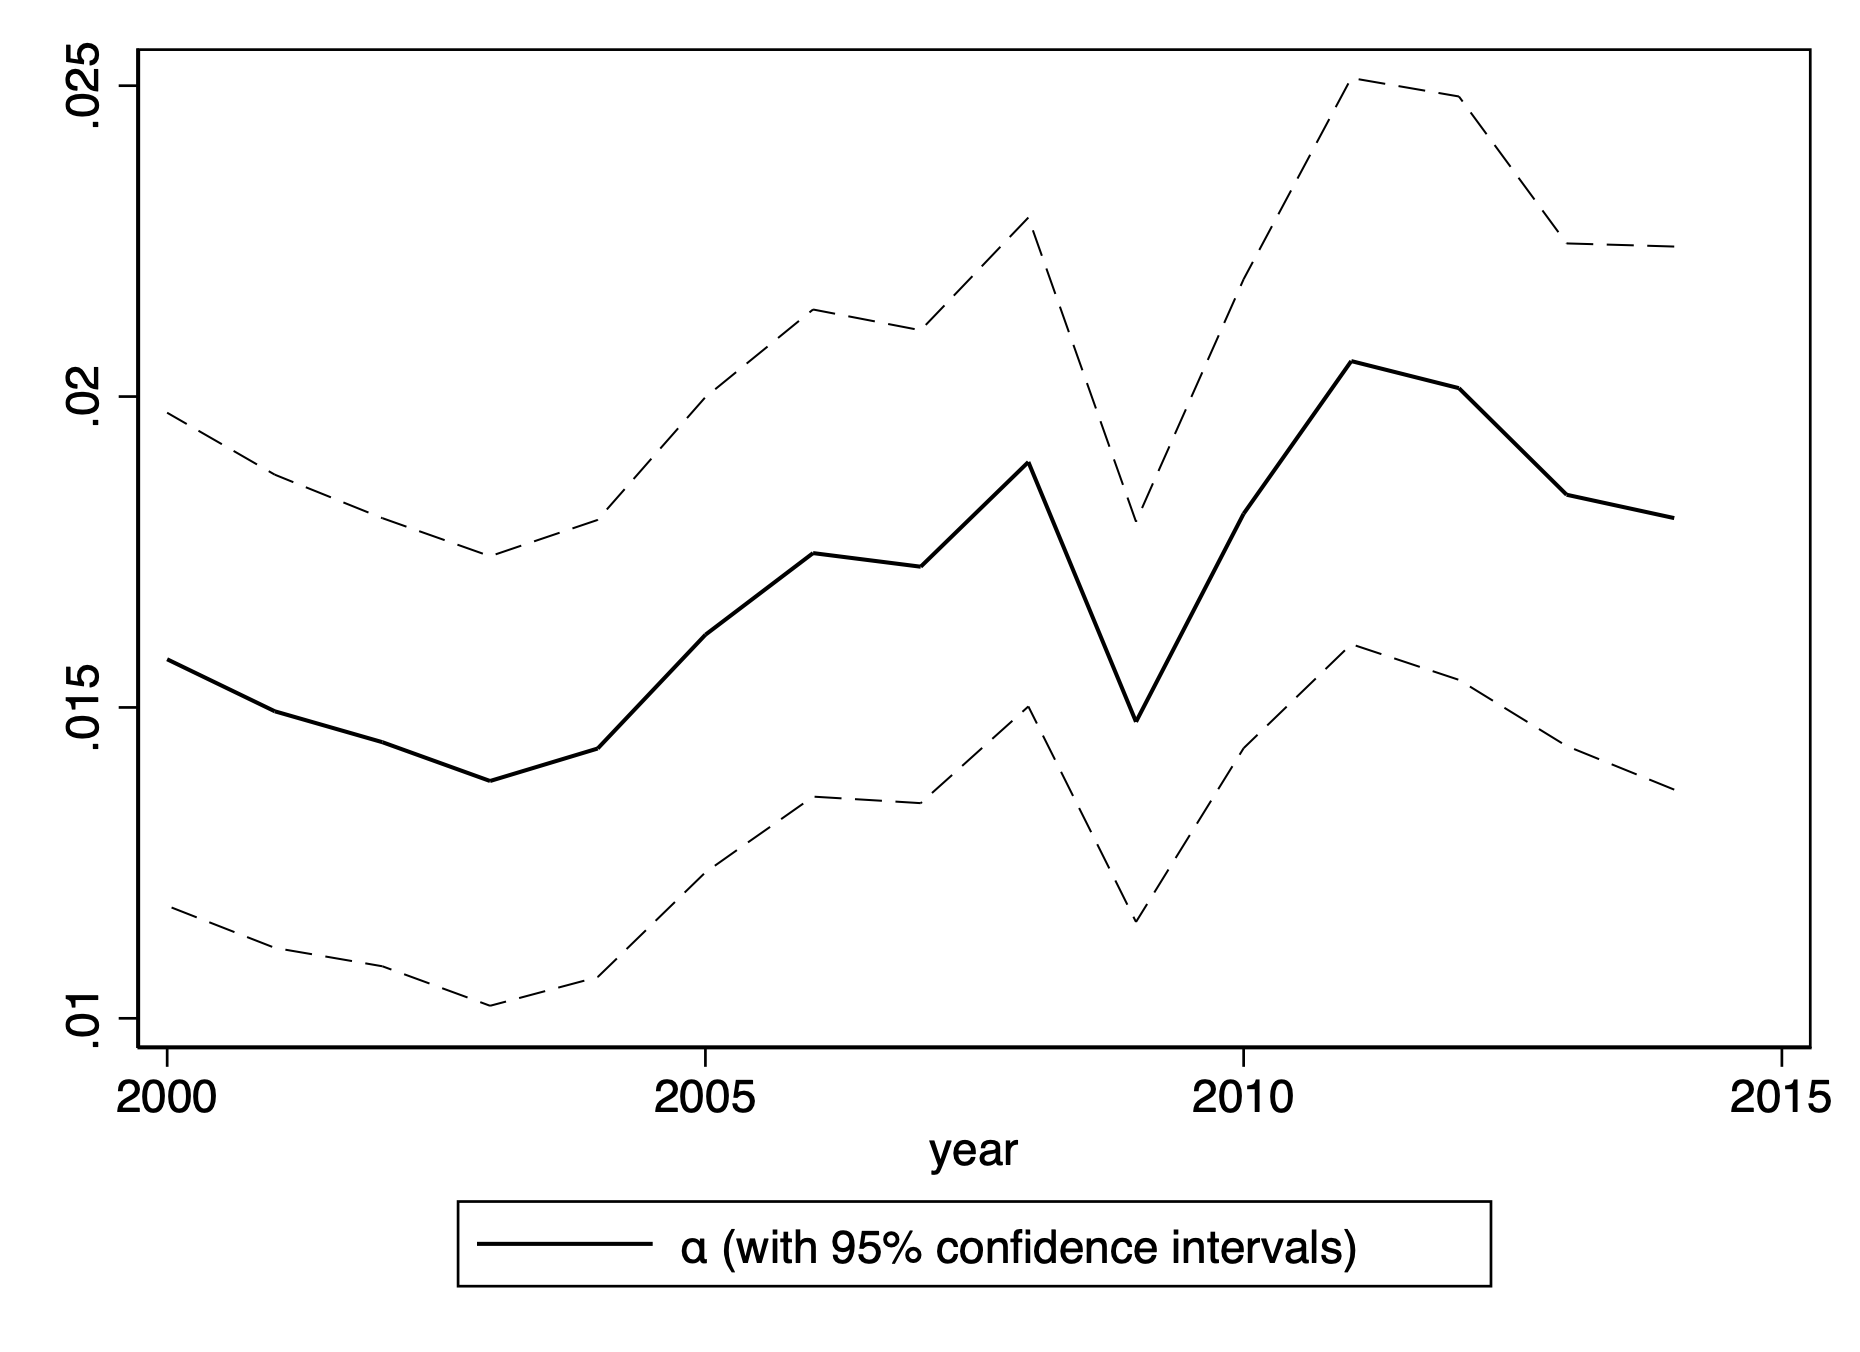
\includegraphics[width=5.0in, height=3.5in]{coef_cst_WIOD_HC.png}\\
\end{tabular}
\label{fig:evolution_cst}
\floatfoot{Sources: WIOD and authors’ calculations}
\end{figure}


We obtain similar results with TiVA (see Online Appendix C). 
% je suggère de retirer cette phrase pour simplifier l'exposé, ou éventuellement d'en faire une note de bas de page
%The functional form might seem a bit counterintuitive (one might expect that the elasticity is affine function of openness as summarized by E1), but the analytical examination of the two-country, one sector case, shows that it is plausible (see Appendix \ref{AnalyticalAppendix}).
Our results suggest that we can approximate the HCE deflator elasticity for the most recent years, using the share of imported goods in household consumption and the share of imported inputs in household consumption of domestic goods. $E1.HC+E2.HC$ is a good predictor of the total effects.
Yet, they cannot be extrapolated in a multiplicative way, as the other effects ($E3.HC+E4.HC$) add to them rather than amplifying them.
They are of similar size for small open economies and large closed ones.
It might be that the small economy counterbalances its small size with its large openness rate and vice versa.\footnote{Although this functional form might seem counterintuitive (one might expect that the elasticity is an affine function of openness as summarized by $E1.HC$), the analytical examination of the two-country, one-sector case shows that it is plausible (see Online Appendix D).}
%Back to the main point, it turns out that we do not gain much by inversing matrixes. Of course, this realization is only possible because we were able to computes $\overline{s}_{i}^{i,HC}$ in the first place. Still, it suggests that we could extrapolate the elasticities for not-yet-released years, as long as we have the share of imported goods in household consumption and the share of imported inputs in household consumption of domestic goods. 

\subsection{Doing without TiVA and WIOD, but keeping Eurostat}
However, even these data ($E1.HC$ and $E2.HC$) are not up-to-date for a large number of countries. 
The share of imports in household final consumption and in intermediate consumption for the production of domestic household final consumption are not routinely computed by national statistical institutes. 
We have to use a proxy. It is easy to identify consumption and intermediary goods imports using UN Comtrade data and the BEC classification. 
While the World Bank provides regular estimates for household consumption, it does not provide an estimate for intermediate consumptions. Eurostat provides estimates for intermediate consumptions in the case of European countries.
%VF comme la source n'est pas précisee je mets en commentaire \footnote{And some others for selected years Eurostat, BEC -- PRÉCISER LA SOURCE}. 
Combining these three data sources, we compute the share of imported consumption goods in household consumption and the share of imported inputs in all inputs. 

We mimick equation \ref{eq:eq7} by equation \ref{eq:eq8}. 
We estimate successive cross-sections of equation \ref{eq:eq8} to check whether the proxy is satisfactory. 

 \begin{equation}
 \begin{array}{llll}
\overline{s}_{i}^{i,HC}= \alpha &+  \beta_1  \frac{\textnormal{imported consumption goods}_i}{\textnormal{household consumption}_i} \\ & +  \beta_2  \left[    \frac{\textnormal{imported intermediate goods}_i}{\textnormal{intermediate consumption}_i}*\frac{\textnormal{domestic consumption goods}_i}{\textnormal{household consumption}_i}\right] +\varepsilon_i 
\end{array} 
\label{eq:eq8}
\end{equation}


In the same way, Figure \ref{fig:evolution_b_reg2} mimicks Figure \ref{fig:evolution_b}. 
The results are less encouraging: the $R^2$ is smaller and declining over time, and the estimated coefficient is not constant.


\begin{figure}[H]
	\centering
	\caption{\footnotesize{\textbf{Evolution of $\beta$ and $R2$ (WIOD) using Eurostat data to approximate E1.HC + E2.HC (limited number of countries)}}}
	\begin{tabular}{c}
		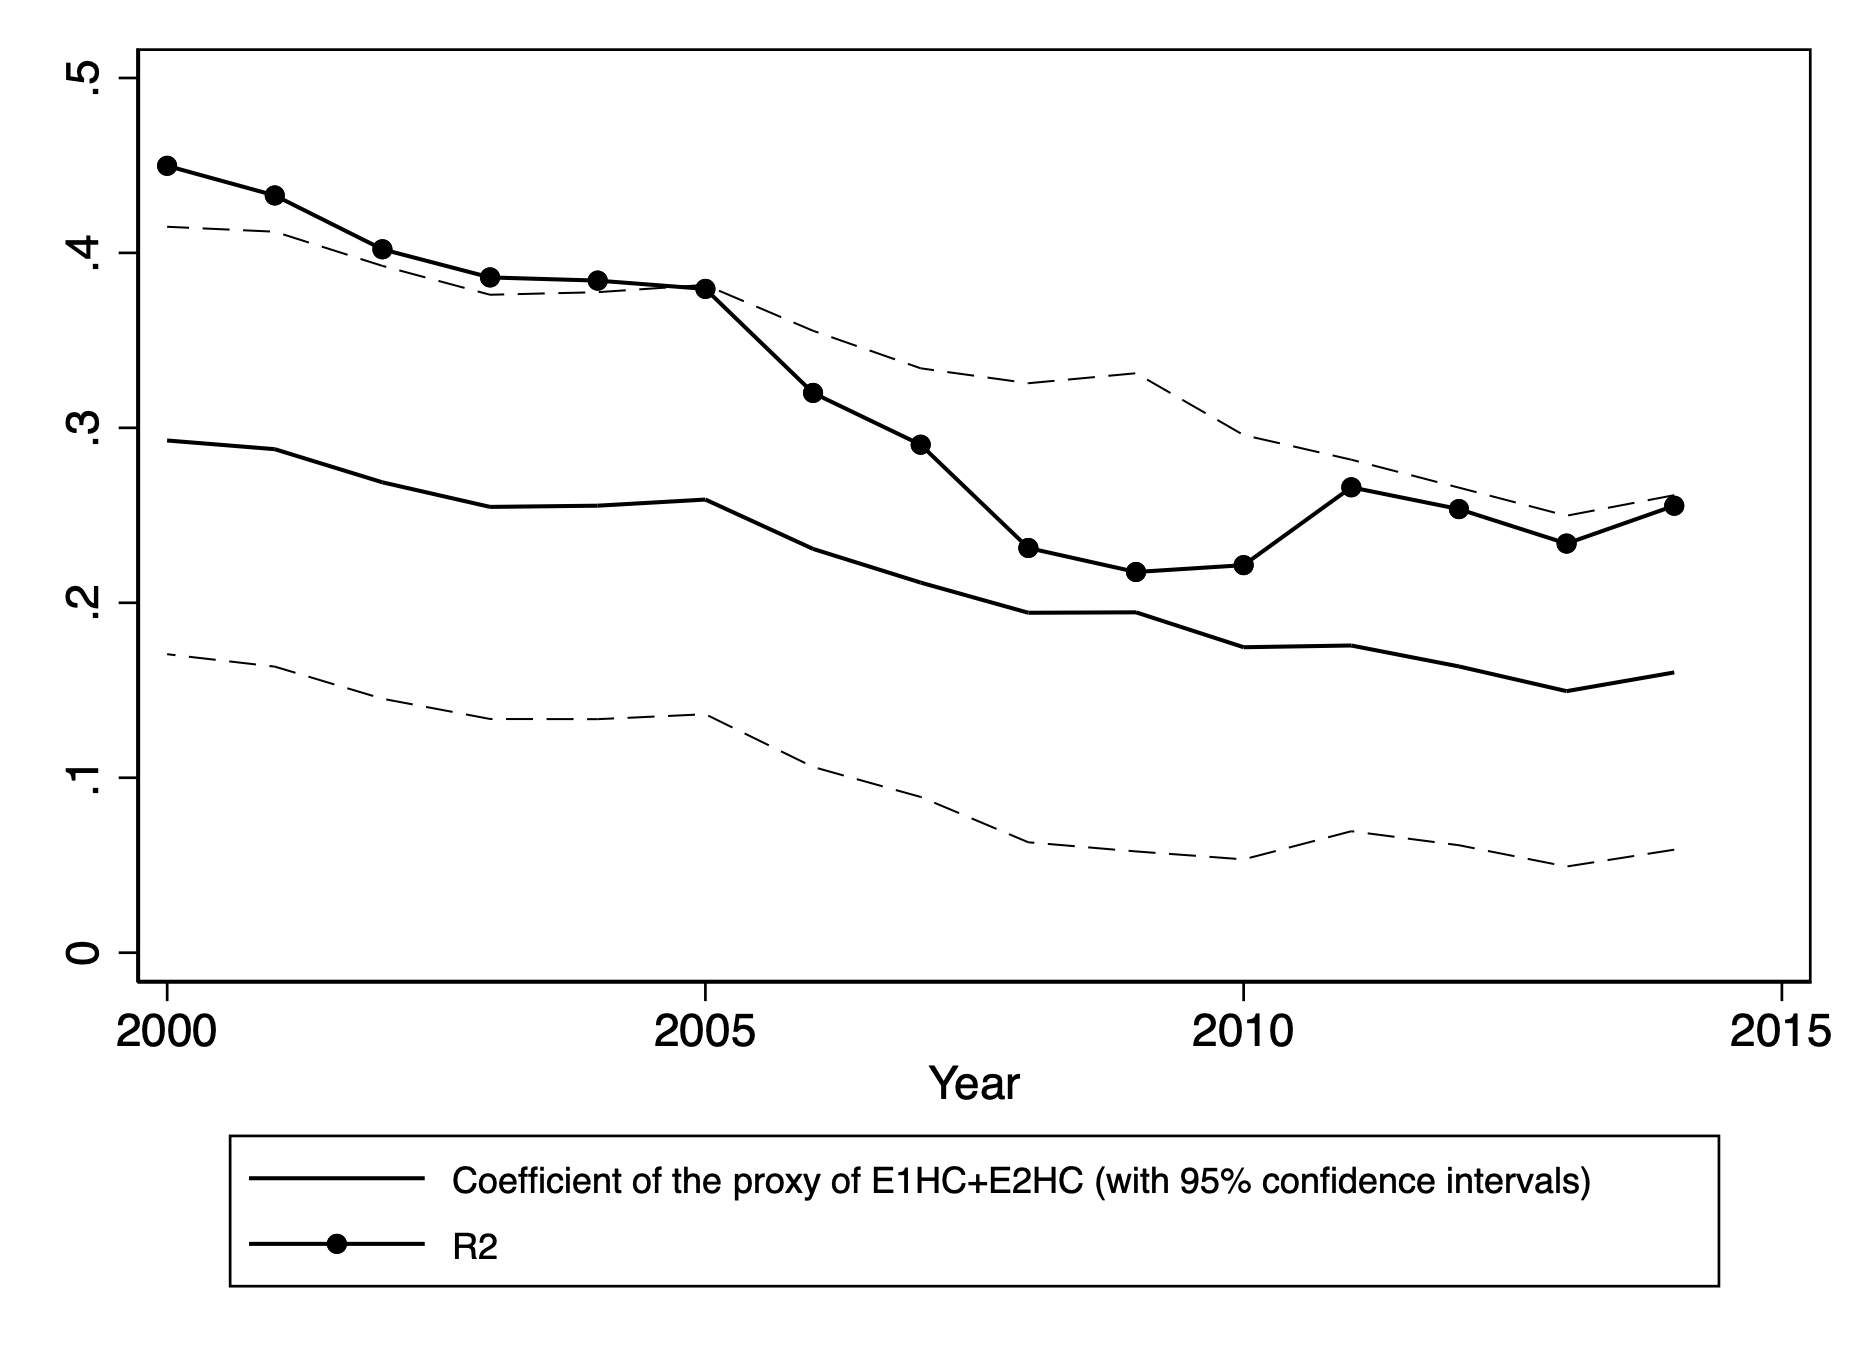
\includegraphics[width=5.0in, height=3.5in]{reg2_beta_WIOD.png}\\
	\end{tabular}
	\label{fig:evolution_b_reg2}
	\floatfoot{Sources: WIOD and authors’ calculations}
\end{figure}

%pas facile à comprendre, je propose de reformuler
%Estimating successive cross-sections of equation \ref{eq:eq8} is a demanding test. 
%In addition, cross-sections do not take advantage of country-specific information.
%To address this issue, we run a panel regression with country-fixed effects.
%We assume that $\beta$ is constant over time for each country $i$ (equation \ref{eq:eq9}).
Yet, estimating successive cross-sections of equation \ref{eq:eq8} is a demanding test to establish a link between the elastiticy computed by PIWIM based on WIOD data and more up-to-date data assembled from various sources.
It does not allow to exploit country-specific information on the determinant of the elasticity.
A less demanding test is to run a panel with country fixed-effects, assuming that $\beta$ is constant over time but that it explains only within-country variations. To take into account year-specific shocks, we add two year-specific variables : the GDP-weighted mean of each variable of interest (see equation \ref{eq:eq9}). 


 \begin{equation}
\begin{array}{llll}
\overline{s}_{i,t}^{i,t,HC}= \alpha &+  \beta_1  \frac{\textnormal{imported consumption goods}_{i,t}}{\textnormal{household consumption}_{i,t}} \\
& + \beta_2 \left[ \frac{\textnormal{imported intermediate goods}_{i,t}}{\textnormal{intermediate consumption}_{i,t}}*\frac{\textnormal{domestic consumption goods}_{i,t}}{\textnormal{houshold consumption}_{i,t}}\right] \\ 
&+  \beta_3 \frac{\textnormal{Total imported consumption goods}_t}{\textnormal{Total household consumption}_t} \\
& + \beta_4  \left[ \frac{\textnormal{Total imported intermediate goods}_t}{\textnormal{Total intermediate consumption}_t}*\frac{\textnormal{Total domestic consumption goods}_t}{\textnormal{Total household consumption}_t} \right] \\ 
& +fe_{i}+\varepsilon_{i,t}
\end{array}
\label{eq:eq9}
\end{equation}

We run the panel regressions for the period 2000 to 2008.
We then estimate the out-of-sample elasticity for each country $i$ for 2014. 
The outcome is close to the elasticity computed with WIOD for 2014 despite a small downward bias (see Figure \ref{fig:panel_pred1}).
Hence, we could use this approach to estimate the HCE deflator elasticity to the exchange rate from 2015 onwards.

\begin{figure}[H]
	\centering
	\caption{\footnotesize{\textbf{Comparing the HCE deflator elasticity in 2014 (WIOD) and the prediction from a panel regression on the 2000-2008 period with fixed effects using Eurostat data.}}}
	\begin{tabular}{c}
		\includegraphics[width=5.0in, height=3.5in]{"resultats_reg2_doigt_mouille_WIOD_pred_6y_trend_no".png}\\
	\end{tabular}
	\label{fig:panel_pred1}
\end{figure}

\subsection{Doing with only World Bank and Comtrade data}
Data on intermediate consumption and household consumption are not available for all countries.
As a result, our regressions only include a limited number of observations.
To expand our panel, we use an even simpler proxy for E1.HC+E2.HC that requires only trade data from Comtrade and GDP data from the World Bank, both available until 2018. 
As a result, we can include many more countries in the new panel (see equation \ref{eq:eq10}).
 \begin{equation}
\begin{array}{llll}
\overline{s}_{i,t}^{i,t,HC}= \alpha & +  \beta_1  \frac{\textnormal{imported consumption goods}_{i,t}}{\textnormal{GDP}_{i,t}} \\ & + \beta_2 \frac{\textnormal{imported intermediate goods}_{i,t}}{\textnormal{GDP}_{i,t}} \\
& +  \beta_3  \frac{\textnormal{Total imported consumption goods}_{t}}{\textnormal{Total GDP}_{t}} \\
& + \beta_4 \frac{\textnormal{Total imported intermediate goods}_{t}}{\textnormal{Total GDP}_{t}} \\
& +fe_{i}+\varepsilon_{i,t}
\end{array}
\label{eq:eq10}
\end{equation}

The out-of-sample prediction remains satisfactory, although the mean and median errors are larger (see Figure \ref{fig:panel_pred2}). 
Our findings are robust to using other databases (revision 3 and revision 4 of TIVA).\footnote{Results are available upon request}


\begin{figure}[!h]
	\centering
	\caption{\footnotesize{\textbf{Comparing the HCE deflator elasticity in 2014 (WIOD) and the prediction from a panel regression on the 2000-2008 period with fixed effects using only World Bank and Comtrade data. }}}
	\begin{tabular}{c}
		\includegraphics[width=5.0in, height=3.5in]{"resultats_reg1_doigt_mouille_WIOD_pred_6y_trend_no".png}\\
	\end{tabular}
	\label{fig:panel_pred2}
	\floatfoot{Sources: WIOD, World Bank, Comtrade and authors’ calculations}
\end{figure}

Using these equations, we can predict the HCE deflator elasticity from 2016 onwards to make up for the lack of WIOTs.
Figure \ref{fig:panel_pred3} shows the predictions. The in-sample predictions seem  rather robust, giving us confidence in the quality of the out-of-sample predictions.


\begin{figure}[H]
	\centering
	\caption{\footnotesize{\textbf{Comparing the output-weighed HCE deflator elasticity to its prediction using only World Bank and Comtrade data.}}}
	\begin{tabular}{c}
		\includegraphics[width=5.0in, height=3.5in]{"predictions_reg1_doigt_mouille_trend_no".png}\\
	\end{tabular}
	\label{fig:panel_pred3}
		\floatfoot{Sources: WIOD, World Bank, Comtrade and authors’ calculations}
\end{figure}





%
%\clearpage
%
%
%\clearpage
%+++++++++++++++++++++++++++++++++++++++++++++++++++++++++
%\subsection{The intensity of import in domestic consumption}
%\label{subsec:intensity}
%
%\begin{figure}[!h]
%\centering
%\caption{\footnotesize{\textbf{The share of imported intermediate and consumer goods and services in private consumption }}}
%\begin{tabular}{c}
%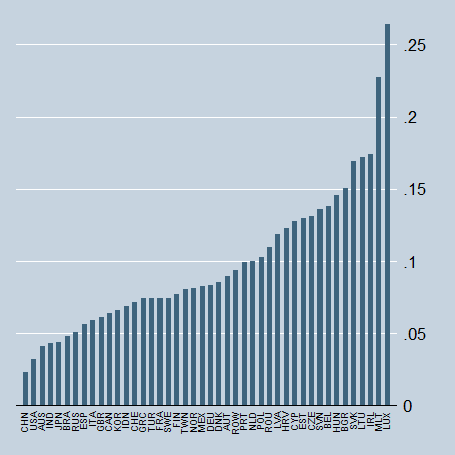
\includegraphics[width=5.0in, height=3.5in]{Graph_ratioimp_wiod_2014}\\
%\floatfoot{Source: WIOD, 2014}.
%\end{tabular}
%\label{fig:ratioimp}
%\end{figure}
%
%Differences in the import intensity across sectors and countries are crucial to our analysis on global nominal spillovers.
%In this section, we present some stylised facts about the import intensity in domestic consumption.
%Using data from the WIOD, we define the import intensity of private consumption as the share of  imported intermediate and final goods and services in total consumption. \\
%Figure \ref{fig:ratioimp} depicts the import intensity  of  household consumption in 2014.
%Not surprisingly, small countries, such as Malta, Luxembourg and Ireland, have the highest import intensity (above 15$\%$), while larger countries, such as Japan, the U.S. and Australia, display a much lower ratio of import intensity.\\
%How has the import intensity of private consumption changed over time? 
%In the Euro area, Figure \ref{fig:ratioimptemp_ze} shows that the import intensity of consumption increased in most member states over the last decade. Following the adoption of the euro, the intensity of import increased between 2000 and 2007 in all countries except the southern economies (Spain, Portugal and Greece). In the years following the Great Recession, the import intensity of consumption kept expanding in the two largest economies of the area (Germany, France), but receded in the countries stricken by the sovereign-debt crisis (Spain, Italy, Portugal and Greece).\\
%Outside of the euro area, Figure \ref{fig:ratioimptemp} shows that the import intensity of consumption has broadly expanded since 2000. 
%In all countries, except China, Croatia, Indonesia and Russia, the import intensity was higher in 2014 than it was in 2000.
%In China, it declined somewhat following the 2008-2009 crisis, reflecting global value chains shortening. In Russia, the intensity of import has been decreasing over the last two decades. 
%\begin{figure}[!h]
%\centering
%\caption{\footnotesize{\textbf{Evolution of the intensity of import in household consumption in the euro area}}}
%\begin{tabular}{c}
%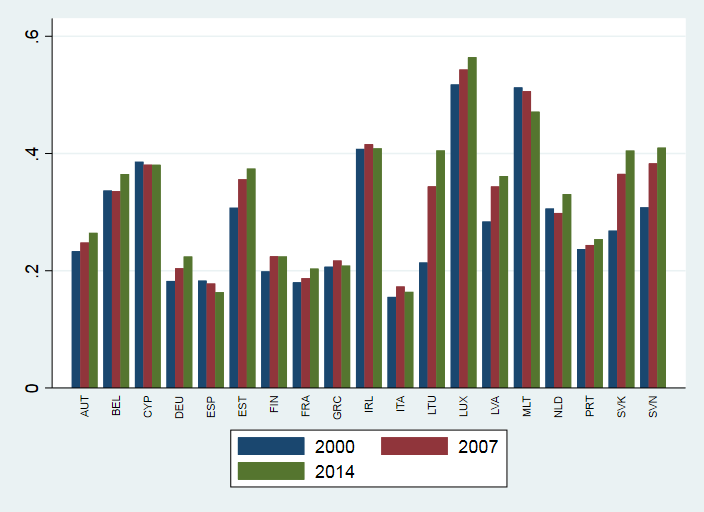
\includegraphics[width=5.0in, height=3.5in]{Graph_ratioimp_WIOD_2000_2014_ze}\\
%\floatfoot{Source: WIOD}.
%\end{tabular}
%\label{fig:ratioimptemp_ze}
%\end{figure}
%
%
%\begin{figure}[!h]
%\centering
%\caption{\footnotesize{\textbf{Evolution of the intensity of import in household consumption}}}
%\begin{tabular}{c}
%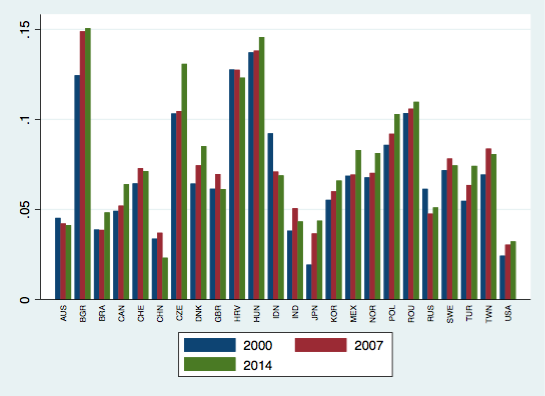
\includegraphics[width=5.0in, height=3.5in]{Graph_ratioimp_WIOD_2000_2014}\\
%\floatfoot{Source: WIOD}.
%\end{tabular}
%\label{fig:ratioimptemp}
%\end{figure}
%
%
%\subsection{The reaction of domestic consumer prices to changes in import prices}
%In this section, we evaluate how domestic consumer prices react to changes in prices of imported intermediate and final goods, the latters being caused by exchange rate fluctuations. 
%We are interested in (\textit{i}) the direct effect of global inflationary shocks, defined as the share of imported final and intermediate goods in domestic consumption (i.e. the import intensity in domestic consumption defined in Section \ref{subsec:intensity}) and (\textit{ii}) the total effect. The latter depends both on the direct effect and on the additional transmission of lower domestic input prices to other sectors of the domestic economy as well as to other countries which occurs during subsequent production cycles. 
%\paragraph{How much of domestic consumer prices' reactions to changes in import prices is explained by the direct effect?}
%
%Figure \ref{fig:ratiodir} depicts how much of the total impact of a change in import prices is explained by the import intensity of household consumption. In other words, Figure \ref{fig:ratiodir} represents the ratio of the direct effect to the total effect.
%In all countries, the direct effect accounts for more than 60$\%$ of the total impact in 2014. 
%%In five economies (India, Indonesia, Luxembourg, Mexico and Turkey), the direct effect explains more than 80$\%$ of the reaction of domestic consumer prices to changes in import prices, which suggests that these countries do not provide much intermediate goods to their partners. 
%For the whole cross-section, the coefficient of correlation between the total and the direct effect is close to unity in 2014.
%
%\begin{figure}[!h]
%\centering
%\caption{\footnotesize{\textbf{Ratio of direct to total effect of domestic consumer prices reactions to changes in import prices}}}
%\begin{tabular}{c}
%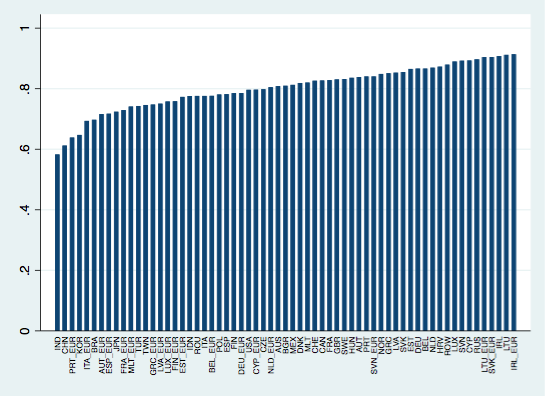
\includegraphics[width=5.0in, height=3.5in]{Graph_ratiodir_WIOD_2014}\\
%\floatfoot{Source: WIOD, 2014}.
%\end{tabular}
%\label{fig:ratiodir}
%\end{figure}
%
%
%\section{The impact of exchange rates fluctuations on the main components of consumer prices}
%\label{sec:prixconsosecteur}
%\paragraph{Differences in the intensity of import use across sectors} 
%In this section, we investigate the import intensity of consumption at the sectoral level. We run the following sectoral regressions (Equation \ref{eq:eq8}) for each sector $j$. 
%
% \begin{eqnarray}
%{S^{HC}_j}=\beta_j  I + c_j +\varepsilon
%\label{eq:eq8}
% \end{eqnarray}
% with ${S^{HC}}$ the impact of the devaluation shock on consumer prices, for each country $i$, and $I$ the vector of country-specific and sector-specific import intensity of consumption.
% 
%
%\begin{figure}[!h]
%\centering
%\caption{\footnotesize{\textbf{Consumer prices elasticity to an exchange rate shock: a sectoral analysis}}}
%\begin{tabular}{c}
%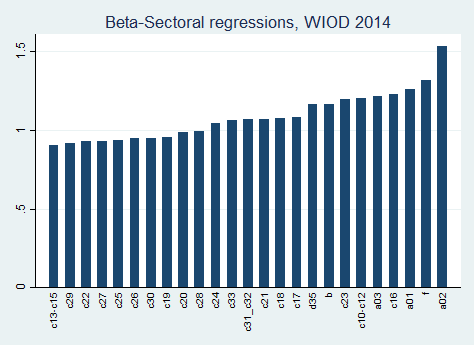
\includegraphics[width=5.0in, height=3.5in]{Graph_beta_2014_Wiod_reg_sec}\\
%\floatfoot{Source: WIOD, 2014. \\
%}
%\end{tabular}
%\label{fig:betasecteur}
%\end{figure}
%
%\begin{figure}[!h]
%\centering
%\caption{\footnotesize{\textbf{Sectoral analysis: R2}}}
%\begin{tabular}{c}
%\includegraphics[width=5.0in, height=3.5in]{Graph_r2_2014_Wiod_reg_sec}\\
%\floatfoot{Source: WIOD, 2014. \\
%}
%\end{tabular}
%\label{fig:betar2}
%\end{figure}

\section{Conclusion}
\label{sec:ccl}
% VF 27 Sept je propose d'enlever la référence aux policy makers, à la BCE etc car le lien me parait bcp trop tenu avec notre papier, cela apparait tout d'un coup et ce n'est pas notre objet. On cite dans l'introduction le débat sur la PC, je pense que c'est suffisant et propose de nous concentrer sur des conclusions factuelles plut^t que sur des références vagues
In this paper, we investigate the role of GVCs for inflation dynamics within a unified framework of input-output databases (WIOT and TIVA) from 1995 to 2018.  
Our main results are threefold.
First, we confirm the importance of Global Value Chains in explaining inflation dynamics.
%GVC cannot be neglected in the debate about the determinants of inflation.
The Household consumption expenditure deflator elasticity to a shock on the domestic currency ranges from 0.05 to 0.35, depending mainly on the openness of countries.
Within the euro area, the range of elasticities is large, adding to the challenges faced by the European Central Bank in stabilising prices throughout the monetary union.
Input-output mechanisms explain a large share of the elasticity, especially for large countries.
Our results are robust to using different databases (WIOD, TiVA 2016 and TiVA 2018).

Second, we show that the direct impact (through imported final goods) and domestic Input-Output linkages (i.e. domestic final goods produced using foreign inputs) account for most of the propagation of an exchange rate shock to domestic prices.
First-round effects explain three-quarters of the propagation of exchange rate shocks to domestic prices.
By contrast, we find a limited role for the second-round effects, i.e. the additional transmission of lower domestic input prices to other sectors of the domestic economy and other countries occurring during subsequent production cycles.
We analyse the contribution of different sectors to the HCE deflator elasticity to an exchange rate shocks. Domestic core inflation (defined as inflation excluding food and energy) accounts for a significant share of the total elasticity, mainly reflecting the weight of domestic services and non-energy industrial goods in total consumption.


Third, we provide a tool to make up for the lack of timely WIOTs. 
The construction of World Input-Output tables is data-demanding and WIOTs are typically released with a lag of several years. 
To address this gap, we use more up-to-date GDP and trade data, which can be easily updated and used to make up for the lack of WIOTs.
We thus provide a tool for approximating the HCE deflator elasticity to an exchange rate shock from 2015 onwards.

%je propose d'enlever la phrase ci-dessous, on le dit déà au début de la conclusion. Il serait plus intéressant d'esquisser des pistes pour prolonger ce papier
%Overall, our results confirm and quantify the usefulness of the Input-Output approach for understanding inflation dynamics, which is key as for monetary policy. 

%%GD20200621Peut-être faudrait-il faire le boulot de la figure 2 pour la période 2016-2019 ???


\newpage
\bibliography{PapiertransmissiondeschocsenVA.bib}

\end{document}
